\documentclass[twoside,11pt]{article}

\usepackage{algorithm}
\usepackage{algpseudocode}
\usepackage{jmlr2e}
\usepackage{amsmath}
\usepackage{booktabs}
\usepackage{array}
\usepackage{lastpage}
\urlstyle{tt}

\newcommand{\R}{\mathbb{R}}
\newcommand{\argmin}{\mathop{\mathrm{argmin}}}
\newcommand{\norm}[1]{\left\lVert #1 \right\rVert}
\newcommand{\fuserplus}{\texttt{fuserplus}}
\DeclareMathOperator{\clip}{clip}

\jmlrheading{1}{2026}{1-\pageref{LastPage}}{4/26}{--}{26-0000}{Agyapong}
\ShortHeadings{Sparse-Graph Solvers for Grouped Fused Regression}{Agyapong}
\firstpageno{1}

\begin{document}

\title{Sparse-Graph Fusion Solvers for Scalable Grouped Regression}

\author{\name Daniel Agyapong \email agyapongdaniel7777@gmail.com \\
       \addr Northern Arizona University\\
       Flagstaff, AZ, USA}

\editor{}

\maketitle

\begin{abstract}
Grouped regression models estimate related but subgroup-specific linear
parameters by combining sparsity with fusion penalties across a graph of
groups. Existing implementations can become expensive when the number of
groups is large, especially when they materialize full pairwise fusion
operators even though the scientific or data-driven fusion graph is sparse.
This paper presents a sparse-graph representation principle for grouped fused
regression: if the statistical objective is defined on a sparse graph, the
optimizer should preserve the same edge set rather than materializing a
complete graph and encoding sparsity through zeros. This principle gives both
an equivalence guarantee for the exact solvers and an immediate complexity
reduction from all-pairs graph construction to active-edge graph construction.
The \fuserplus package implements this principle for L1- and L2-fused
grouped regression. The L1
operator solver evaluates the same smoothed proximal-gradient updates using
only active graph edges, while the chain-specialized solver replaces a general
graph by a DFS-induced chain when maximum computational efficiency is
preferred over exact graph fidelity. The L2 solver reformulates the augmented
regression design using active-edge triplets rather than dense all-pair
construction before calling \texttt{glmnet}.
Across public grouped regression benchmarks, the exact L1 operator reproduces
the legacy predictive accuracy while reducing median runtime by 2.26x and
median peak memory by 10.7\% on the completed benchmark suite. The chain
variant gives a median 3.26x runtime reduction with an accuracy tradeoff.
Across 19 L2 benchmark datasets, active-edge construction has no systematic
loss in test error and reduces median fit time by 14.9x. The implementation
includes package tests, documented solver routines, benchmark manifests, and
the CSV summaries used to regenerate the paper figures.
\end{abstract}

\begin{keywords}
  fused lasso, grouped regression, sparse graphs, optimization, R package
\end{keywords}

\section{Introduction}

Many regression problems contain a natural grouping variable: patients may
belong to disease subtypes, schools to districts, countries to regions, or
time series to meters. Fitting a separate model in each group ignores shared
signal, whereas fitting one global model ignores heterogeneity. Grouped fused
regression addresses this middle ground by estimating one coefficient vector
per group and penalizing differences between coefficient vectors along a graph
of group relationships.

Let $X_g \in \R^{n_g \times p}$ and $y_g \in \R^{n_g}$ denote the data for
group $g$, and let $\beta_g \in \R^p$ be that group's linear coefficient
vector. For a graph $G=(V,E)$ over $k$ groups with nonnegative edge weights
$w_{gh}$, the estimators considered in this paper have the form
\begin{equation}
\label{eq:model}
  \min_{\beta_1,\ldots,\beta_k}
  \sum_{g=1}^{k} \frac{1}{2 n_g} \norm{y_g - X_g \beta_g}_2^2
  + \lambda \sum_{g=1}^{k} \norm{\beta_g}_1
  + \gamma \sum_{(g,h)\in E} w_{gh} \Omega(\beta_g-\beta_h).
\end{equation}
For the L1 fused model, $\Omega(u)=\norm{u}_1$; for the L2 fused model,
$\Omega(u)=\frac{1}{2}\norm{u}_2^2$ after the standard augmented-design
reformulation. Optional group-specific intercepts are included in the
software implementation but are excluded from sparsity and fusion penalties.
This formulation is a direct descendant of the lasso, fused lasso, grouped
and elastic-net regularization, graph-structured fused optimization, and
subgroup regression models reviewed below. The L1 solver uses the standard
Nesterov smoothing strategy for nonsmooth penalties \citep{nesterov2005smooth}.

The central computational issue is a mismatch between the statistical object
and the solver representation. A complete graph has $k(k-1)/2$ edges, but
practical graphs are frequently chains, trees, nearest-neighbor graphs, or
domain-informed sparse networks. If the objective is defined on only $m$
active edges, a solver that builds all pairwise fusion constraints and then
uses zero weights for inactive edges changes the computational scaling of the
problem without changing its statistical content. This matters as $k$ grows:
the modeling assumption is sparse, but the legacy representation is still
quadratic.

The contribution of this paper is to make the sparse graph a first-class
object in the optimizer. The key idea is to represent the fused-regression
objective in a way that respects the graph on which the penalty is defined.
First, the paper gives an exact active-edge L1 operator form that evaluates
the smoothed proximal-gradient fusion term only over active edges. Second, it
gives an exact active-edge L2 augmented-design construction that emits sparse
triplets only for nonzero graph edges before delegating the regularized
regression path to \texttt{glmnet} \citep{glmnet}. Third, it separates these
exact reformulations from approximation-oriented solver modes, including a
chain-specialized L1 approximation that collapses a graph to $k-1$ chain edges
using a depth-first traversal, motivated by chain-structured fused lasso
solvers. The result is a reusable design pattern for multi-task fused
regression and other graph-penalized models whose penalties decompose over
graph edges.

The main contributions are:
\begin{itemize}
\item a sparse-graph representation principle for grouped fused regression
solvers;
\item exact active-edge L1 and L2 reformulations that preserve the legacy
objective while avoiding zero-weight all-pair construction;
\item a clear separation between exact sparse-graph solvers and approximate
high-efficiency chain variants;
\item empirical comparisons showing when fused regression improves over
unfused \texttt{glmnet} baselines and when active-edge construction improves
over legacy fused solvers; and
\item an open R implementation with benchmark scripts, manifests, and
figure-generation artifacts.
\end{itemize}

The implementation is provided in the R package \fuserplus. The current
benchmark suite uses public grouped regression datasets and synthetic scaling
experiments to compare prediction error, wall time, and peak resident memory.
The results show that graph-aware construction can deliver substantial runtime
and memory reductions without changing the statistical objective for the exact
operator and L2 variants.

\section{Related Work}

The fused lasso extends the lasso by combining sparsity with penalties on
ordered coefficient differences \citep{tibshirani1996lasso,tibshirani2005fused}.
This places grouped fused regression in a broader family of structured
regularizers, including the elastic net, group lasso, generalized lasso, and
graph trend filtering
\citep{zou2005elastic,yuan2006group,tibshirani2011genlasso,wang2016graphtf}.
Specialized algorithms for one-dimensional signal approximation, including
path algorithms for the fused lasso signal approximator, exploit the ordered
chain structure of that problem \citep{hoefling2010path}. Split Bregman and
ADMM methods provide another important optimization line for nonsmooth fused
penalties \citep{ye2011split,boyd2011admm}. General graph fusion is more
flexible but computationally harder because the penalty couples many
coefficient blocks.

Graph-structured multi-task regression extended these ideas to arbitrary task
graphs and developed smoothed proximal-gradient methods for the general fused
lasso \citep{chen2010graph,chen2012smoothing}. Related multi-task and
scientific applications use graph-guided fusion for eQTL mapping, additive
modeling, gene regulatory network inference, and subgroup-specific regression
\citep{chen2012twograph,petersen2016flam,omranian2016gene}.
Network lasso methods \citep{hallac2015network}, graph trend filtering,
DFS fused lasso denoising \citep{tansey2018dfs}, and
k-nearest-neighbor fused lasso estimators \citep{padilla2020adaptive} further
emphasize that the graph itself is part of the modeling problem: it may come
from prior knowledge, distances between groups, or other data-driven
structure.

The present work focuses on how grouped fused regression objectives should be
represented and solved when the graph is sparse. This is more than an
implementation detail: the graph is part of the modeling assumption, and a
dense all-pairs representation discards that assumption at the computational
layer. The active-edge constructions developed below restore the intended
edge-level representation while preserving the legacy objective in the exact
L1 and L2 cases.

Table~\ref{tab:software-comparison} summarizes the closest available software
ecosystem. The closest package overall is the R package \texttt{fuser}, because
it implements the same subgroup-regression interface and L1/L2 fusion family
that \fuserplus extends. Outside R, the
closest package by statistical model is the MATLAB MMT library for
graph-guided multi-task lasso, which uses coefficient matrices and explicit
task graphs but targets multi-task learning rather than the
\texttt{X}, \texttt{y}, \texttt{groups}, \texttt{G} subgroup API.
The closest Python package by penalty
language is \texttt{yaglm}, which supports structured penalties including
fused and generalized lasso, but is a general penalized-GLM framework rather
than a subgroup-fusion regression package. Packages such as
\texttt{genlasso} and \texttt{Lasso.jl} overlap with the fused/generalized
lasso optimization language, but not with the paired L1/L2 subgroup-fusion
workflow considered here. Additional packages
provide useful but narrower reference points: \texttt{flsa} targets fused
lasso signal approximation, \texttt{extlasso} provides fused-lasso penalized
linear regression, \texttt{smoothedLasso} implements smoothed L1 penalty
operators, \texttt{penalized} supports fused-lasso penalties in several
regression families, and \texttt{CVXPY} can express total-variation or fused
penalties through convex modeling atoms. Citations for each package are given
directly in the table.

\begin{table}[t]
\centering
\scriptsize
\caption{Closest software relatives to \fuserplus. The main distinction is
that \fuserplus targets subgroup regression with inputs
$(X,y,\mathrm{groups},G)$, both L1 and L2 fusion, and sparse-graph solver
variants for scaling.}
\label{tab:software-comparison}
\begin{tabular}{@{}>{\raggedright\arraybackslash}p{0.16\textwidth}
>{\raggedright\arraybackslash}p{0.12\textwidth}
>{\raggedright\arraybackslash}p{0.29\textwidth}
>{\raggedright\arraybackslash}p{0.34\textwidth}@{}}
\toprule
Package & Language & Closest overlap & Difference from \fuserplus \\
\midrule
\texttt{Lasso.jl} \citep{lassojl} & Julia &
Lasso paths plus fused lasso and trend filtering support. &
Primarily regression paths, one-dimensional fused lasso, and trend filtering;
not a graph-based subgroup-fusion package. \\
MMT \citep{mmtmanual} & MATLAB &
Graph-guided multi-task lasso with coefficient matrices and task graphs. &
Multi-task learning library rather than subgroup-regression API; includes
feature-graph and task-graph fusion with a different optimizer. \\
\texttt{CVXPY} \citep{cvxpy} & Python &
Convex modeling language with total-variation atoms and custom fused penalties. &
Useful for prototyping formulations; not a packaged subgroup-fusion estimator
or benchmarked solver workflow. \\
\texttt{yaglm} \citep{yaglm} & Python &
General penalized-GLM framework with structured penalties including fused
lasso. &
Closest Python penalty toolbox, but not a dedicated subgroup L1/L2 fusion
package. \\
\texttt{extlasso} \citep{extlassopkg} & R &
Fused-lasso penalized linear regression with $\lambda_1$ and $\lambda_2$
penalties. &
Fuses neighboring coefficients in a single regression model; not graph fusion
across subgroup-specific coefficient vectors. \\
\texttt{flsa} \citep{flsapkg} & R &
Path algorithm for the fused lasso signal approximator, including connected
difference structures. &
Signal-approximation focus with response vector or image-like inputs; not
subgroup coefficient fusion for regression predictors. \\
\texttt{fuser} \citep{fuserpkg,dondelinger2020joint} & R &
Same subgroup fused-regression family; same legacy L1/L2 solver interface. &
Closest overall baseline; \fuserplus adds active-edge and chain variants
focused on sparse-graph runtime and memory scaling. \\
\texttt{genlasso} \citep{genlassopkg} & R &
Generalized-lasso and fused-lasso path algorithms. &
General path solver; does not provide the subgroup-regression package
workflow or paired L1/L2 fusion API. \\
\texttt{penalized} \citep{penalizedpkg} & R &
L1, fused-lasso, and L2 penalized estimation for GLMs and Cox models. &
Broad penalized-model package; not designed around subgroup graphs or
active-edge L1/L2 fusion construction. \\
\texttt{smoothedLasso} \citep{smoothedlassopkg} & R &
Nesterov-smoothed L1 penalty operators, including fused-lasso helpers. &
Penalty/operator framework rather than a grouped-regression package with
benchmarked L1/L2 sparse-graph solvers. \\
\bottomrule
\end{tabular}
\end{table}

Figures~\ref{fig:concept-l1} and~\ref{fig:concept-l2} summarize the main
computational distinction between the legacy fused-regression representation
and the sparse-graph representation used in \fuserplus. In both cases the
statistical model is defined by a graph on the $k$ groups, with an edge
weight indicating how strongly two subgroup coefficient vectors should be
encouraged to agree. The legacy construction first expands this modeling graph
into a dense algebraic object over many group pairs. That expansion is benign
for small $k$, but it becomes the dominant cost when the intended graph is
sparse, because computation is then driven by the number of possible group
pairs rather than by the number of modeled edges.

Figure~\ref{fig:concept-l1} describes the L1 fusion case. The nonsmooth
penalty is represented by an operator that maps the coefficient matrix to
absolute coefficient differences across fused group pairs. The full-edge
operator stores and applies constraints for the expanded group-pair
construction, whereas the active-edge operator stores only the $m$ nonzero
edges of the graph. The right panel is therefore not just a complexity
summary: it illustrates the change in the dominant algebraic object from a
group-expanded constraint matrix to a sparse edge list, which changes the
fusion-side scaling from depending on powers of $k$ to depending linearly on
the number of graph edges.

Figure~\ref{fig:concept-l2} gives the analogous picture for L2 fusion. In the
quadratic case, fusion can be represented by augmenting the regression design
with pseudo-observations that penalize differences between subgroup
coefficients. The legacy construction emits augmented rows for the expanded
set of group pairs; the active-edge construction emits sparse triplets only for
edges with nonzero fusion weight. Thus the same modeling graph produces a much
smaller linear-algebra problem whenever $m \ll k^2$. These two figures motivate
the solver descriptions in Section~\ref{sec:solvers} and the scaling
experiments reported below: the central question is whether preserving the
edge-level graph representation yields the same fitted objective at lower
runtime and memory cost.

\begin{figure}[t]
  \centering
  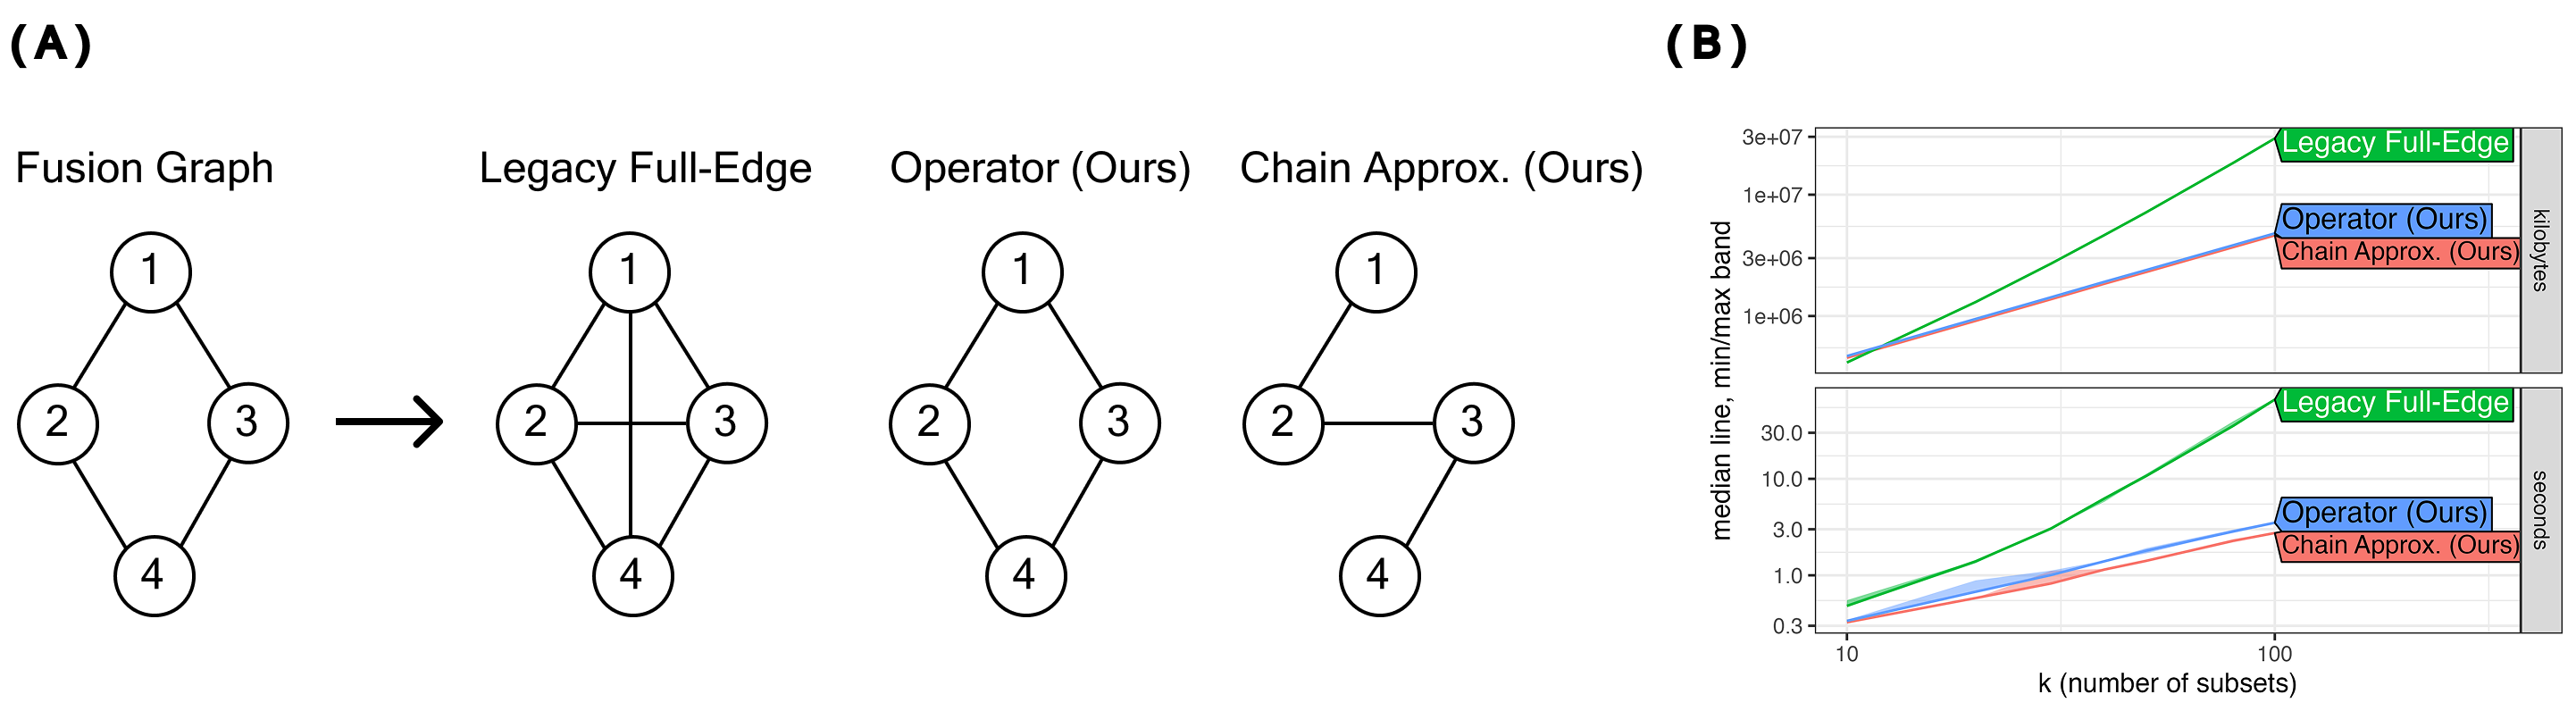
\includegraphics[width=.95\textwidth]{figures/concept1.png}
  \caption{Conceptual overview of L1 sparse-graph fusion. A: fusion graph
  construction. The legacy full-edge construction associated with
  \citet{dondelinger2020joint} forms a combined constraint matrix over all
  group pairs, while the active-edge operator works directly on the sparse
  graph. B: asymptotic complexity. The synthetic example fixes $p=120$ and
  $n_{\mathrm{group,train}}=35$, so at $k=100$ the total training sample size
  is $n=3500$. With a sparse chain graph and fixed remaining hyperparameters,
  the active-edge representation changes the dominant fusion cost from
  $O(pk^3)$ to $O(pm)$.}
  \label{fig:concept-l1}
\end{figure}

\begin{figure}[t]
  \centering
  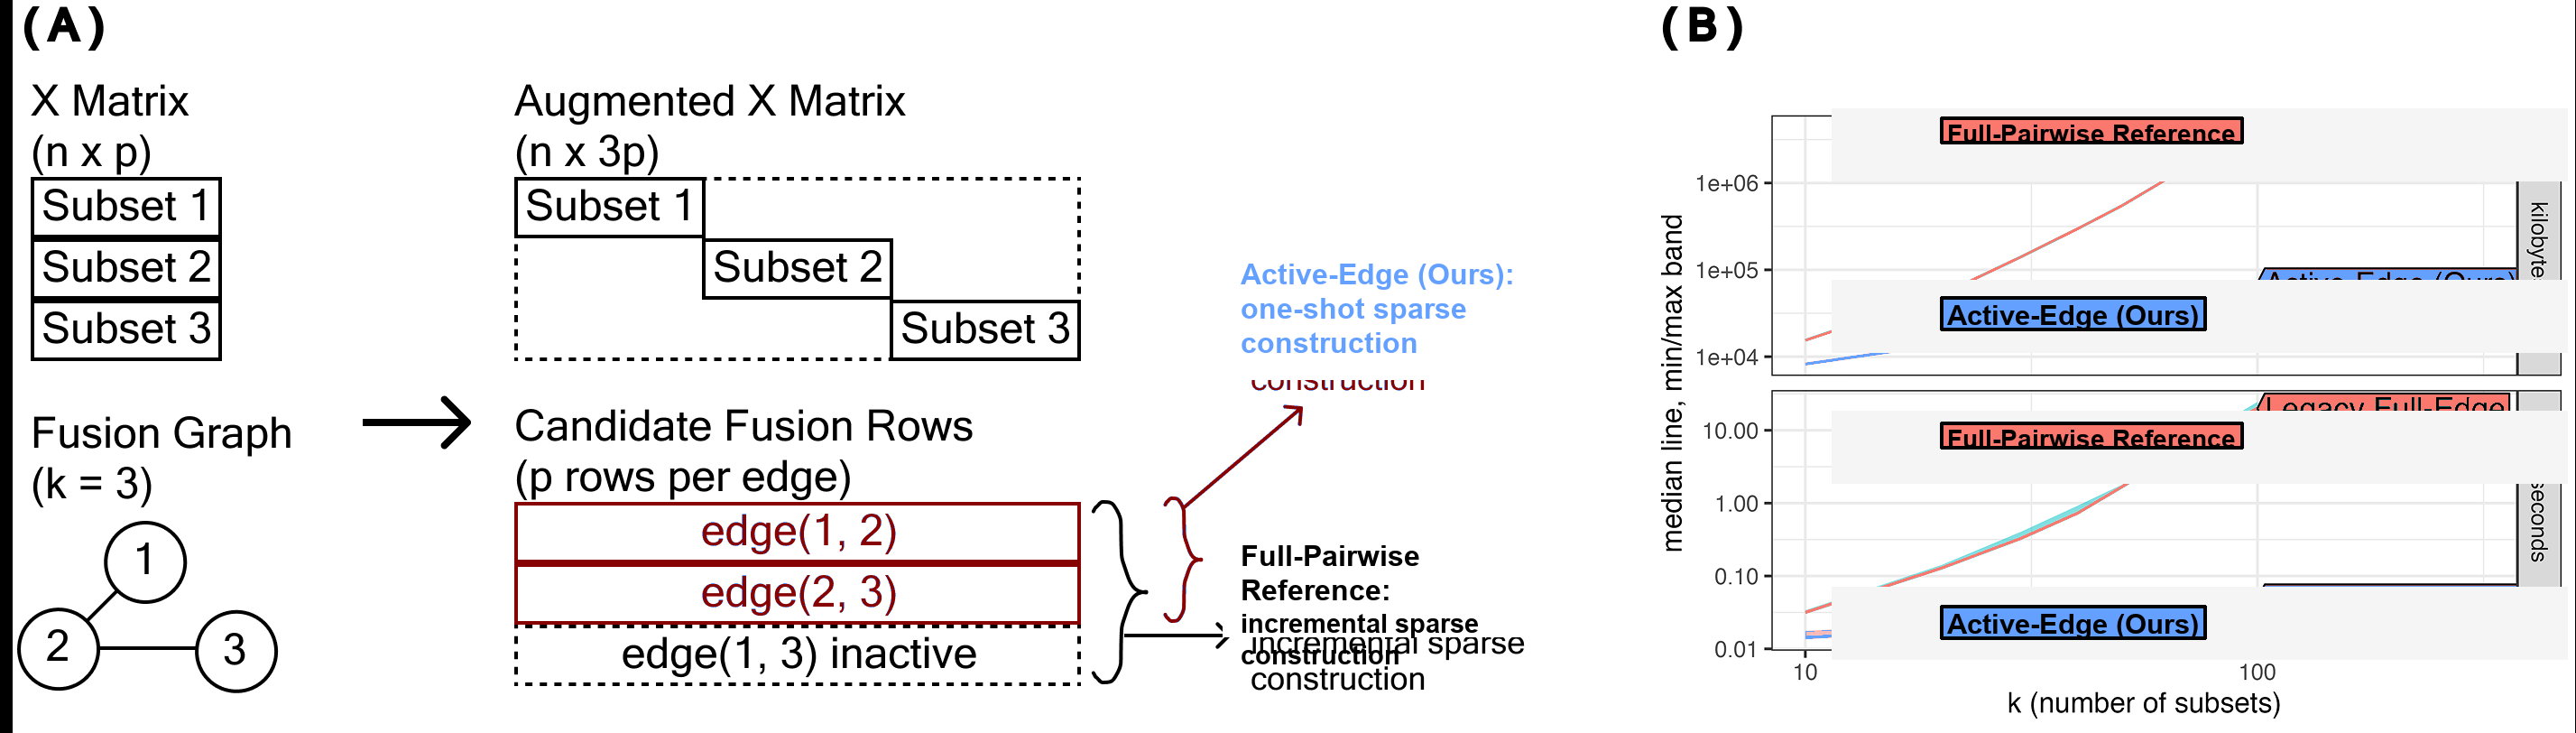
\includegraphics[width=.95\textwidth]{figures/concept2.png}
  \caption{Conceptual overview of L2 sparse-graph fusion. A: augmented matrix
  construction. The legacy full-edge construction associated with
  \citet{dondelinger2020joint} forms augmented rows for all group pairs, while
  the active-edge builder emits only sparse triplets for graph edges with
  nonzero weight. B: asymptotic complexity. The synthetic example fixes
  $p=120$ and $n_{\mathrm{group,train}}=35$, so at $k=100$ the total training
  sample size is $n=3500$. With a sparse chain graph and fixed remaining
  hyperparameters, active-edge construction changes the dominant fusion-block
  cost from $O(pk^2)$ to $O(pm)$.}
  \label{fig:concept-l2}
\end{figure}

\section{Model and Legacy Computation}

The L1 solver in \fuserplus follows a smoothed proximal-gradient strategy for
Equation~\ref{eq:model}. Let $B=[\beta_1,\ldots,\beta_k]$ be the $p \times k$
coefficient matrix. The legacy implementation builds a constraint matrix with
columns for sparsity and fusion constraints, then uses a smoothed dual
approximation to compute the gradient contribution of the nonsmooth penalty.
The update has the generic accelerated form
\begin{align}
  A^\star &= \Pi_{[-1,1]}\left(\frac{B C}{\mu}\right),\\
  \nabla f_\mu(B) &= \nabla \ell(B) + A^\star C^\top,\\
  B^{t+1} &= W^t - L^{-1}\nabla f_\mu(B^t),
\end{align}
where $C$ encodes the sparsity and fusion operators, $\mu$ is the smoothing
parameter, $L$ is a Lipschitz bound, and $W^t$ is the accelerated iterate.
When $C$ contains all group pairs, storage and multiplication include
$O(pk^2)$ fusion terms for a complete representation.

More explicitly, the L1 implementation uses the dual identity
$|z|=\max_{|a|\leq 1} az$ and replaces the nonsmooth absolute-value terms by
clipped smoothed duals. For sparsity and active fusion edges this gives
\[
  A_s^\star = \clip\left(\frac{\lambda B_s}{\mu}, -1, 1\right),
  \qquad
  A_{uv}^\star =
  \clip\left(\frac{\gamma w_{uv}(\beta_u-\beta_v)}{\mu}, -1, 1\right),
\]
where $B_s$ excludes intercept rows. The code uses the step-size upper bound
\[
  L_U =
  \lambda_{\max}
  + \frac{\lambda^2+2\gamma^2 d_{\max}^{(w)}}{\mu},
\]
with $\lambda_{\max}=\sum_g \lambda_{\max}(X_g^\top X_g/n_g)$ under scaled
group losses and weighted maximum degree proxy $d_{\max}^{(w)}$ for the
active fusion graph.

\begin{proposition}[Equivalence of dense and active-edge L1 gradients]
\label{prop:l1-equivalence}
\leavevmode\par\noindent
Fix a weighted graph $G$ and let $E$ denote the edges with positive weight.
For smoothing parameter $\mu>0$, suppose the dense smoothed proximal-gradient
implementation includes one fusion column for every pair but assigns zero
weight to inactive pairs. The active-edge operator implementation computes
exactly the same smoothed fusion gradient as the dense implementation after
removing the zero-weight columns.
\end{proposition}

\begin{proof}
For edge $e=(u_e,v_e,w_e)$, the dense fusion column has nonzero endpoint
entries with opposite signs. Its smoothed dual contribution is
$p_e=\clip((\gamma w_e/\mu)(\beta_{u_e}-\beta_{v_e}),-1,1)$. Multiplying the
dense constraint matrix by this dual vector adds $\gamma w_e p_e$ to column
$u_e$ and subtracts $\gamma w_e p_e$ from column $v_e$. Algorithm
\ref{alg:active_edge_operator} performs exactly these two scatter operations
for each active edge and performs no operation for inactive zero-weight
columns. Summing over edges therefore gives the same gradient contribution.
\end{proof}

\begin{algorithm}[t]
\caption{Legacy Full-Edge Smoothed APG (\texttt{old\_l1})}
\label{alg:old_l1}
\begin{algorithmic}[1]
\Require grouped data, $G$, $\lambda,\gamma,\mu,T,\varepsilon$
\State Construct full fusion matrix $C_{\mathrm{fusion}}\in\R^{k\times \binom{k}{2}}$
\State Construct $C=[\lambda I_k,\gamma C_{\mathrm{fusion}}]$
\State Initialize $B^{(0)}=0,\;W^{(0)}=0,\;S^{(0)}=0$
\For{$t=1,\dots,T$}
  \State Compute $\nabla \ell(B^{(t-1)})$ groupwise
  \State $A^\star\gets
  \clip\!\left([B_s^{(t-1)}C_s,\;B_f^{(t-1)}C_f]/\mu,-1,1\right)$
  \State $\nabla r_\mu(B^{(t-1)})\gets A^\star C^\top$
  \State $G_t \gets \nabla \ell(B^{(t-1)})+\nabla r_\mu(B^{(t-1)})$
  \State Compute $L_U$ from the dense max-degree proxy
  \State Update $\tilde B^{(t)},S^{(t)},W^{(t)}$
  \If{$\norm{\tilde B^{(t)}-B^{(t-1)}}_1<\varepsilon p$}
    \State \textbf{break}
  \EndIf
  \State $B^{(t)}\gets \tilde B^{(t)}$
\EndFor
\State Soft-threshold non-intercept rows by $\lambda/n_g$
\State \Return $\hat B$
\end{algorithmic}
\end{algorithm}

The L2 solver uses a different reduction. It constructs an augmented response
and design matrix,
\[
  \tilde y =
  \begin{bmatrix} y \\ 0 \end{bmatrix}, \quad
  \tilde X =
  \begin{bmatrix} X_{\mathrm{block}} \\ X_{\mathrm{fusion}} \end{bmatrix},
\]
where $X_{\mathrm{block}}$ is block diagonal over groups and
$X_{\mathrm{fusion}}$ contains, for each group pair, rows proportional to
\[
  \sqrt{\gamma w_{gh}}(\beta_g-\beta_h).
\]
The resulting lasso problem is passed to \texttt{glmnet}. A full all-pairs
construction creates $O(p k^2)$ fusion rows even when only $m=|E|$ edges are
active.

\begin{proposition}[Equivalence of active-edge L2 augmented rows]
\label{prop:l2-equivalence}
For a fixed graph $G$, penalty $\gamma$, and scaling convention, the
active-edge L2 augmented design is equivalent to the legacy all-pairs
augmented design after deleting all zero-weight pair rows and applying a row
permutation.
\end{proposition}

\begin{proof}
Each nonzero edge $(u,v)$ contributes $p_{\mathrm{eff}}$ augmented rows with
$+\sqrt{\gamma w_{uv}}$ in coefficient block $u$ and
$-\sqrt{\gamma w_{uv}}$ in coefficient block $v$, with zero augmented
response. The active-edge builder constructs exactly these rows using sparse
triplets. Inactive pair rows have zero weight in the legacy construction and
therefore add zero residual contribution to the augmented least-squares
objective. Removing them and permuting the remaining rows leaves the
objective minimized by \texttt{glmnet} unchanged.
\end{proof}

\begin{proposition}[Representation-dependent graph cost]
\label{prop:complexity}
\leavevmode\par\noindent
Let $m$ be the number of nonzero graph edges and let $q=\binom{k}{2}$. In one
L1 smoothed-gradient evaluation, a dense all-pairs operator performs fusion
work proportional to $pq$ after construction, whereas the active-edge operator
performs fusion work proportional to $pm$. In the L2 augmented-design
construction, the fusion block decreases from $pq$ rows to $pm$ rows.
\end{proposition}

\begin{proof}
For L1 fusion, each edge contributes one $p$-dimensional coefficient
difference and one $p$-dimensional scatter back to the incident groups. A
dense pairwise representation contains $q$ candidate edges, including zero
weight inactive pairs, while the active-edge representation iterates only over
the $m$ nonzero edges. For L2 fusion, each edge contributes
$p_{\mathrm{eff}}$ augmented rows, one for each penalized coefficient
coordinate. Deleting zero-weight pairs therefore reduces the fusion block from
$p_{\mathrm{eff}}q$ rows to $p_{\mathrm{eff}}m$ rows, up to the intercept
convention.
\end{proof}

\section{Sparse-Graph Solvers}
\label{sec:solvers}

\subsection{Exact L1 Operator Solver}

The exact L1 operator solver replaces the dense fusion matrix representation
with edge lists $(u_e,v_e,w_e)_{e=1}^m$. At each iteration, the solver computes
the fusion differences only on active edges,
\[
  D_e = \beta_{u_e}-\beta_{v_e},
  \quad
  P_e = \Pi_{[-1,1]}\left(\frac{\gamma w_e D_e}{\mu}\right),
\]
and scatters $\gamma w_e P_e$ back to the incident group columns with opposite
signs. The sparsity part of the update remains unchanged. This representation
has the same objective and first-order updates as the active-edge version of
the legacy smoothed proximal-gradient solver, but the fusion work scales with
$pm$ rather than $pk^2$.

The implementation also supports block processing of edges. This is a practical
memory safeguard for large $p$ or $m$, since intermediate edge-difference
matrices can otherwise dominate the working set. The operator solver is
therefore intended as the general exact path for sparse graphs.

\paragraph{Active-edge gradient assembly.}
The operator implementation initializes $\Delta_f=0$ and loops over active
edges $e=1,\ldots,m$. For each edge, it computes
$d_e=\beta_{u_e}-\beta_{v_e}$ and
$p_e=\clip((\gamma w_e/\mu)d_e,-1,1)$, then performs the endpoint updates
\[
  \Delta_f(:,u_e) \leftarrow \Delta_f(:,u_e)+\gamma w_e p_e,
  \qquad
  \Delta_f(:,v_e) \leftarrow \Delta_f(:,v_e)-\gamma w_e p_e.
\]
The accumulated matrix $\Delta_f$ is the fusion contribution added to the
likelihood and sparsity gradients in the accelerated update.

\paragraph{Optimization algorithm.}
The implementation used in the experiments is the following active-edge APG
procedure. It is the central exact L1 routine in \fuserplus.
\begin{algorithm}[t]
\caption{Active-Edge Operator APG (\texttt{operator})}
\label{alg:active_edge_operator}
\begin{algorithmic}[1]
\Require grouped data, edge list $E$, $\lambda,\gamma,\mu,T,\varepsilon$
\State Initialize $B^{(0)}=0,\;W^{(0)}=0,\;S^{(0)}=0$
\For{$t=1,\dots,T$}
  \State Compute groupwise likelihood gradient $\nabla \ell(B^{(t-1)})$
  \State $A_s^\star \gets \clip(\lambda B_s^{(t-1)}/\mu,-1,1)$
  \State Initialize fusion accumulator $\Delta_f \gets 0$
  \For{each edge $e=(u_e,v_e,w_e)\in E$}
     \State $d_e \gets \beta_{u_e}^{(t-1)}-\beta_{v_e}^{(t-1)}$
     \State $p_e \gets \clip((\gamma w_e/\mu)d_e,-1,1)$
     \State $\Delta_f(:,u_e) \gets \Delta_f(:,u_e)+\gamma w_e p_e$
     \State $\Delta_f(:,v_e) \gets \Delta_f(:,v_e)-\gamma w_e p_e$
  \EndFor
  \State $G_t \gets \nabla \ell(B^{(t-1)}) + \lambda A_s^\star + \Delta_f$
  \State Compute $L_U$ on active graph; update $\tilde B^{(t)},S^{(t)},W^{(t)}$
  \If{$\norm{\tilde B^{(t)}-B^{(t-1)}}_1 < \varepsilon p$}
    \State \textbf{break}
  \EndIf
  \State $B^{(t)}\gets \tilde B^{(t)}$
\EndFor
\State Soft-threshold non-intercept rows by $\lambda/n_g$
\State \Return $\hat B$
\end{algorithmic}
\end{algorithm}

\subsection{Chain-Specialized L1 Approximation}

The chain-specialized solver is a deliberately approximate method. It builds a
depth-first traversal of a maximum spanning tree or of the thresholded graph,
reorders the groups along that traversal, and keeps only the $k-1$ adjacent
chain edges. The fusion operator can then be computed with vectorized adjacent
differences:
\[
  D_j = \beta_j-\beta_{j+1}, \quad j=1,\ldots,k-1.
\]
The vectorized implementation forms
\[
  D = B_{:,1:(k-1)} - B_{:,2:k}, \qquad
  P = \clip((\gamma/\mu)D\operatorname{diag}(w),-1,1),
\]
and accumulates $\gamma P\operatorname{diag}(w)$ on neighboring chain
endpoints.
This reduces the edge budget to the minimum needed to connect the groups. It
does not optimize the same objective as the original graph unless the graph is
already the selected chain. It is useful when the main objective is maximum
speed and memory reduction and the user is willing to accept a small loss in
graph fidelity.

\paragraph{Optimization algorithm.}
The chain-specialized code first builds the DFS/MST order and adjacent chain
weights, then runs a separate vectorized APG routine rather than calling the
general edge loop:
\begin{algorithm}[t]
\caption{Chain-Specialized APG (\texttt{chain\_specialized})}
\label{alg:chain_specialized}
\begin{algorithmic}[1]
\Require grouped data, $G$, chain settings, $\lambda,\gamma,\mu,T,\varepsilon$
\State Build DFS/MST chain order $\pi$ and adjacent chain weights $(w_1,\dots,w_{k-1})$
\State Reorder groups by $\pi$; initialize $B^{(0)}=0,\;W^{(0)}=0,\;S^{(0)}=0$
\For{$t=1,\dots,T$}
  \State Compute groupwise likelihood gradient $\nabla \ell(B^{(t-1)})$
  \State $A_s^\star\gets\clip(\lambda B_s^{(t-1)}/\mu,-1,1)$
  \State $D\gets B^{(t-1)}_{:,1:(k-1)}-B^{(t-1)}_{:,2:k}$
  \State $P\gets \clip\!\left(\frac{\gamma\,D\operatorname{diag}(w)}{\mu},-1,1\right)$
  \State $C\gets \gamma\,P\operatorname{diag}(w)$
  \State Initialize fusion accumulator $\Delta_f\gets 0$
  \State $\Delta_f(:,1:(k-1)) \mathrel{+}= C,\qquad
  \Delta_f(:,2:k) \mathrel{-}= C$
  \State $G_t\gets \nabla \ell(B^{(t-1)})+\lambda A_s^\star+\Delta_f$
  \State Compute chain $L_U$ and update $\tilde B^{(t)},S^{(t)},W^{(t)}$
  \If{$\norm{\tilde B^{(t)}-B^{(t-1)}}_1<\varepsilon p$}
    \State \textbf{break}
  \EndIf
  \State $B^{(t)}\gets \tilde B^{(t)}$
\EndFor
\State Soft-threshold non-intercept rows by $\lambda/n_g$
\State Reorder columns back to original group order
\State \Return $\hat B$
\end{algorithmic}
\end{algorithm}

\subsection{Active-Edge L2 Augmented Design}

The L2 active-edge solver preserves the augmented-design strategy but changes
how the design is built. Instead of allocating all pairwise fusion blocks and
then assigning zero-weight rows, it finds the upper-triangular nonzero entries
of $G$ and builds sparse triplets only for those edges. The same scaling
semantics as the legacy implementation are used:
\[
  \sqrt{\gamma(n+n_{\mathrm{fusion}})}\sqrt{w_{gh}}
\]
multiplies the positive and negative entries in the fusion rows. The final
augmented design is passed to \texttt{glmnet} with the same lambda correction
factor as the original wrapper.

This change leaves the fitted objective unchanged for a given active graph but
reduces the number of constructed fusion rows from $p k(k-1)/2$ to $pm$.
The largest expected gains occur when $m \ll k(k-1)/2$.

\paragraph{Optimization algorithm.}
The L2 path uses \texttt{glmnet} after building an augmented sparse regression
problem:
\begin{algorithm}[t]
\caption{L2 via Augmented Design and \texttt{glmnet}}
\label{alg:l2_augmented_design}
\begin{algorithmic}[1]
\Require grouped data $(X,y,\mathrm{groups})$, graph $G$, $\lambda,\gamma$, scaling settings
\State Build block-diagonal design $X_{\mathrm{block}}$ over groups
\State Build fusion rows $X_{\mathrm{fusion}}\gets\textsc{BuildFusionRows}(G)$
\State Scale fusion block by $\sqrt{\gamma(n+n_{\mathrm{fusion}})}$
\State Form augmented system $\tilde X=[X_{\mathrm{block}};X_{\mathrm{fusion}}]$, $\tilde y=[y;0]$
\State Fit $\theta$ with \texttt{glmnet} on $(\tilde X,\tilde y)$ using $\lambda$
\State Reshape $\theta$ to $B\in\R^{p_{\mathrm{eff}}\times k}$
\State \Return $B$
\end{algorithmic}
\end{algorithm}

\begin{algorithm}[t]
\caption{\textsc{BuildFusionRows}$(G)$ for Active-Edge L2}
\label{alg:l2_fusion_rows}
\begin{algorithmic}[1]
\Require graph $G$
\State Extract active edges $E=\{(u,v):u<v,\;G_{uv}\ne 0\}$
\State Initialize sparse triplet lists for $X_{\mathrm{fusion}}$
\For{each active edge $(u,v)\in E$}
  \State Add $p_{\mathrm{eff}}$ rows with $+\sqrt{w_{uv}}$ on block $u$
  \State Add matching entries with $-\sqrt{w_{uv}}$ on block $v$
\EndFor
\State \Return $X_{\mathrm{fusion}}$
\end{algorithmic}
\end{algorithm}

\begin{table}[t]
\centering
\caption{Dominant representation costs of the solver variants. Here
$n$ is total sample size, $p$ is feature count, $k$ is group count, $m=|E|$
is the number of active fusion edges, $q=\binom{k}{2}$, $T$ is the L1
iteration count, and $I$ is the number of \texttt{glmnet} sweeps. The table
isolates graph-representation costs and omits lower-order constants from R
bookkeeping and solver overhead.}
\label{tab:complexity}
\begin{tabular}{lll}
\toprule
Method & Time & Memory \\
\midrule
legacy L1 full edge & $O(T(np+pkq))$ & $O(np+pk+pq+kq)$ \\
L1 active-edge operator & $O(T(np+pm))$ & $O(np+pk+m)$ \\
L1 chain-specialized & $O(T(np+pk))$ & $O(np+pk)$ \\
legacy L2 full pairwise & $O(I(np+pq))$ & $O(np+pq)$ \\
L2 active-edge & $O(I(np+pm))$ & $O(np+pm)$ \\
\bottomrule
\end{tabular}
\end{table}

\section{Experimental Design}

\subsection{Datasets}

The repository contains a processed grouped-regression inventory of 22 public
datasets. Across this inventory, the number of observations ranges from 200
to 220,908, the number of features from 3 to 100, and the number of groups
from 10 to 3,058. Sources include UCI datasets, Rdatasets mirrors, Our World
in Data CO2 data, World Bank indicators, NYC TLC trip records, OpenML, and
other public sources documented in the repository.

The completed L1 benchmark summary covers 12 datasets with five outer folds
per dataset. The L2 benchmark summary covers 19 datasets with five outer
folds per dataset, including 11 datasets with at least 50 groups. The
reported figures and tables are generated from CSV summaries under
\texttt{build/hpc} and \texttt{build/hpc/l2\_knn}; the plotting artifacts are
stored under \texttt{inst/figures} and copied into the paper source tree.

Table~\ref{tab:datasets} lists the complete union of datasets that appear in
the final L1 and L2 result summaries used by this paper. The remaining
processed datasets are retained in the repository for future experiments but
are not included in the reported final benchmark panels.
The \texttt{SubsetType} column reports the semantic unit defining the
subgroups in the regression problem.

\begin{table}[t]
\centering
\scriptsize
\caption{Public grouped-regression datasets used in the reported real-data
benchmark panels. The columns report total observations $n$, feature count
$p$, group count $k$, and semantic subgroup type after preprocessing in this
repository.}
\label{tab:datasets}
\begin{tabular}{@{}>{\raggedright\arraybackslash}p{0.24\textwidth}rrr
>{\raggedright\arraybackslash}p{0.14\textwidth}
>{\raggedright\arraybackslash}p{0.21\textwidth}@{}}
\toprule
Dataset & $n$ & $p$ & $k$ & \texttt{SubsetType} & Source \\
\midrule
\path{beijing_air_quality} & 180,000 & 14 & 12 & stations &
UCI Beijing air quality \citep{uci_beijing} \\
\path{communities_crime} & 1,991 & 100 & 43 & states &
UCI Communities and Crime \citep{uci_communities} \\
\path{electricity_load} & 200,000 & 3 & 120 & meters &
UCI Electricity Load \citep{uci_electricity} \\
\path{nyc_tlc_yellow_2022} & 200,000 & 9 & 82 & pickup zones &
NYC TLC yellow taxi records \citep{nyctlc2022} \\
\path{owid_co2} & 7,763 & 4 & 164 & countries &
Our World in Data CO2 \citep{owidco2} \\
\path{radon_minnesota} & 916 & 5 & 82 & counties &
PyMC Minnesota radon example \citep{pymcexamples} \\
\path{rdatasets_cigar} & 1,380 & 7 & 46 & states &
Rdatasets, \texttt{plm::Cigar} \citep{rdatasets} \\
\path{rdatasets_crime4} & 630 & 57 & 90 & counties &
Panel crime data \citep{cornwell1994crime} \\
\path{rdatasets_dietox} & 861 & 6 & 72 &
pigs & Dietox pig-growth data \citep{lauridsen1999dietox} \\
\path{rdatasets_empluk} & 1,031 & 5 & 140 & firms &
Employment panel data \citep{arellano1991panel} \\
\path{rdatasets_exam_inner_london} & 4,057 & 7 & 64 &
schools & Inner London exam data \citep{goldstein1993exam} \\
\path{rdatasets_fatalities} & 336 & 32 & 48 & states &
Rdatasets, \texttt{AER::Fatalities} \\
\path{rdatasets_grunfeld} & 200 & 3 & 10 & firms &
Rdatasets, \texttt{plm::Grunfeld} \\
\path{rdatasets_guns} & 1,173 & 11 & 51 & states &
Rdatasets, \texttt{AER::Guns} \\
\path{rdatasets_hsb82} & 7,185 & 6 & 160 & schools &
High-school multilevel data \citep{raudenbush2002hlm} \\
\path{rdatasets_ratpupweight} & 322 & 3 & 27 & litters &
Rdatasets, \texttt{nlme::RatPupWeight} \\
\path{sarcos_openml} & 44,484 & 21 & 10 & response bins &
OpenML SARCOS 43873 \citep{openmlsarcos} \\
\path{school_ilea} & 7,185 & 10 & 160 & schools &
\texttt{nlme} school data \citep{pinheiro2000mixed} \\
\path{world_bank_wdi} & 10,830 & 4 & 229 & economies &
World Development Indicators \citep{worldbankwdi} \\
\bottomrule
\end{tabular}
\end{table}

\subsection{Evaluation Protocol}

All reported real-data results use grouped outer cross-validation with five
stratified folds and random seed 20260221. Splits are made at the observation
level while preserving group representation where possible; datasets with
very small groups are filtered using a minimum group size of seven. All graph
construction, hyperparameter selection, and standardization are performed
inside the outer-training fold so that the held-out test fold is not used in
model selection.

For each outer fold, the baseline sparsity parameter is selected on the
outer-training data by \texttt{cv.glmnet} with three inner folds and
\texttt{lambda.min}. A separate inner train-validation split of the
outer-training data selects the fusion strength $\gamma$ by validation RMSE.
The final model is then refit on the full outer-training fold using the
selected $\lambda$ and $\gamma$ and evaluated on the held-out outer fold. The
featureless baseline predicts the training-fold mean for the corresponding
response. Runtime is measured for the fit stage, and memory is the peak
resident set size recorded by the worker process.

\subsection{Graph Construction and Hyperparameters}

The real-data benchmark constructs a data-driven group graph from training
data, following the use of graph-based relationships and k-nearest-neighbor
fusion graphs in prior work \citep{hallac2015network,padilla2020adaptive}.
Group centroids are computed on the outer-training fold, a k-nearest-neighbor
graph is formed from centroid distances, inverse-distance weights are used,
and connectivity is enforced by adding nearest inter-component links.
The manifest records $k=5$ nearest neighbors, inverse-distance weights, and
MST-style connectivity augmentation. This follows the general idea that graph
structure should encode similarity between groups rather than defaulting to a
complete graph.

Each dataset is evaluated with five outer folds. The regularization parameter
$\lambda$ is warm-started from \texttt{cv.glmnet}; the fusion parameter
$\gamma$ is selected from the grid
\[
  10^{-6}, 10^{-5}, 10^{-4}, 10^{-3}, 10^{-2}, 10^{-1}.
\]
The L1 optimization tolerance is $10^{-5}$ with a maximum of 1200 iterations
in the HPC manifest. Runs use intercepts for L1 models, no feature scaling
inside the L1 solver, standardized inputs for benchmark construction, an
edge-block size of 256 for the operator implementation, and the adaptive
operator fallback threshold recorded in the manifest. The L2 panel uses the
same outer-fold and graph protocol with the L2 solvers.

\subsection{Compared Methods}

For L1 fusion, the benchmark compares the legacy full construction
(\texttt{old\_l1}), the exact active-edge operator solver
(\texttt{operator}), the chain approximation (\texttt{chain\_specialized}),
and a featureless baseline. For L2 fusion, the benchmark compares the legacy
augmented design (\texttt{old\_l2}), the active-edge augmented design
(\texttt{new\_l2}), and the featureless baseline.

The exact comparisons are intentionally conservative. The operator and
active-edge L2 methods are compared against legacy implementations using the
same graph, outer folds, selected hyperparameters, and prediction pipeline.
Thus the reported differences isolate representation and construction costs,
not changes in the statistical model. The chain-specialized L1 method is
reported separately because it changes the graph and is therefore an
approximation rather than an exact replacement.

\section{Results}

\subsection{Changepoint Structure Relative to Glmnet}

Before comparing solver representations, it is useful to show a setting where
fusion is statistically useful relative to unfused \texttt{glmnet} baselines.
We generated an ordered-group regression problem with $k=60$ groups,
$p=20$ predictors, and piecewise-constant coefficient paths with changepoints
after groups 20 and 40. Each group has 25 training observations for fitting,
10 validation observations for tuning, and 80 test observations. The graph is
the chain over ordered groups. We compare a pooled \texttt{glmnet} model, a
group-specific interaction \texttt{glmnet} model with no fusion, and the L1
fused model on the same chain graph.

The pooled \texttt{glmnet} baseline cannot represent group-specific
changepoints. The group-specific \texttt{glmnet} baseline can represent
heterogeneity but has no mechanism to share strength across adjacent groups,
so its fitted paths are noisy and contain many spurious jumps. The fused L1
model uses the graph penalty to recover the piecewise-constant structure. In
this controlled example it has the lowest test RMSE and coefficient error, and
it produces exactly two large jumps, both at the true changepoints.

\begin{figure}[t]
  \centering
  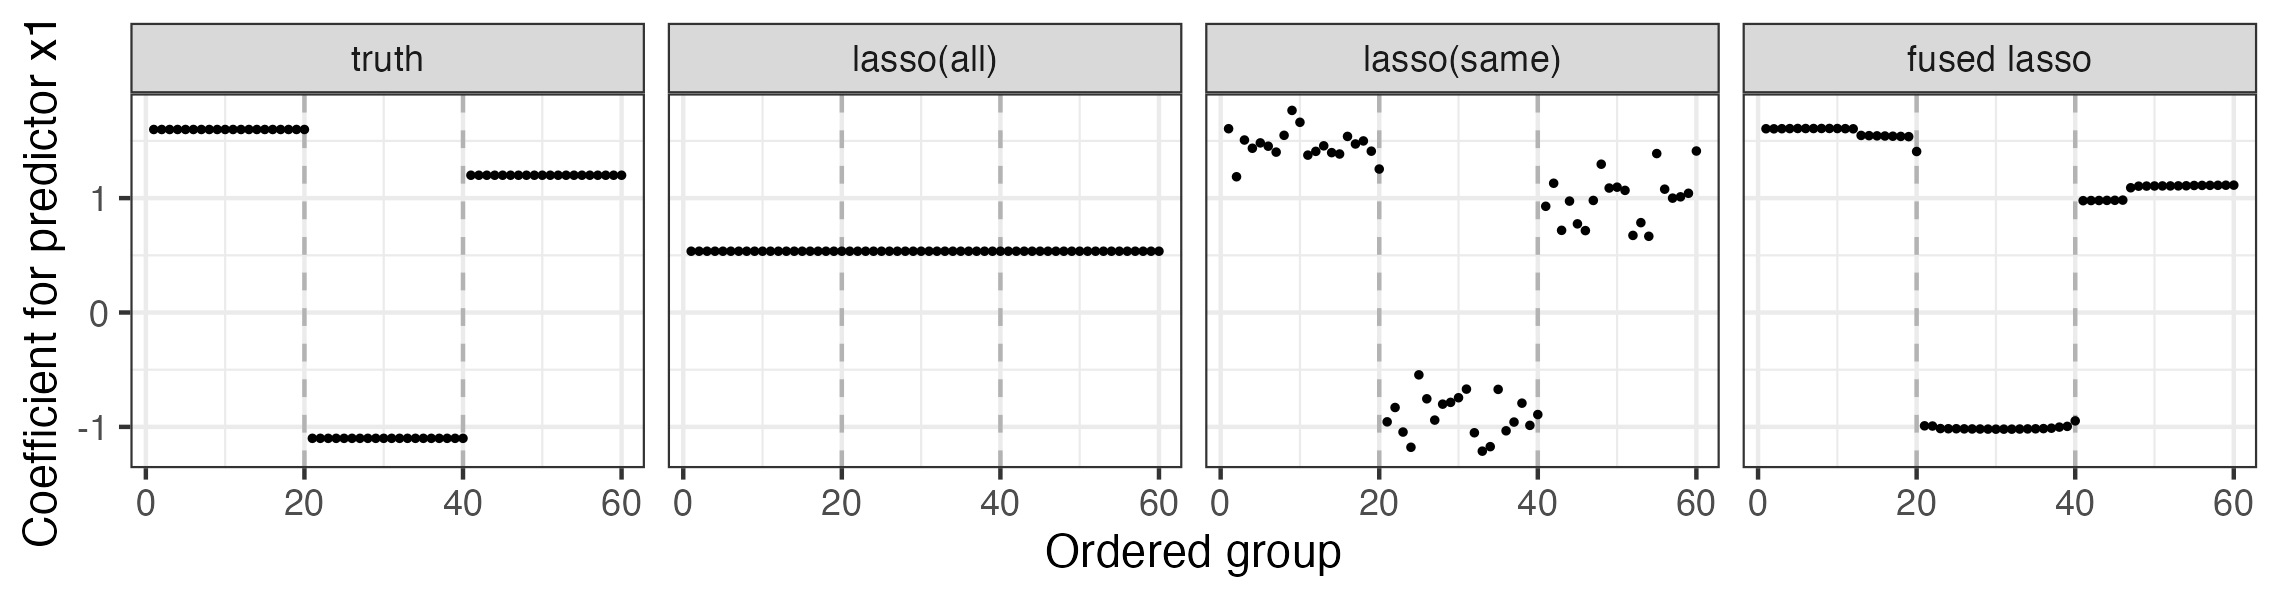
\includegraphics[width=.9\textwidth]{figures/changepoint_fused_vs_glmnet.png}
  \caption{Controlled changepoint example comparing fused regression with
  \texttt{glmnet} baselines. Dashed vertical lines mark the true changepoints.
  Pooled \texttt{glmnet} underfits group heterogeneity, group-specific
  \texttt{glmnet} overfits noisy group-level paths, and the fused L1 model
  recovers the piecewise-constant coefficient structure.}
  \label{fig:changepoint-glmnet}
\end{figure}

\subsection{Spatial Hotspot Structure Relative to Glmnet}

A second use case replaces the one-dimensional chain by a two-dimensional
spatial graph. We generated an $8\times 8$ grid of groups with 4-neighbor
adjacency, $p=16$ predictors, and two contiguous hotspot regions whose
coefficient vectors differ from the background. Each group has 25 training
observations for fitting, 10 validation observations for tuning, and 70 test
observations. This setting mimics county-, sensor-, image-, or station-level
regression problems where local regions share regression structure and
boundaries are sparse.

The pooled \texttt{glmnet} baseline again cannot represent local
heterogeneity. The group-specific \texttt{glmnet} baseline can represent
heterogeneity, but without a spatial fusion penalty it produces fragmented
coefficient maps and many spurious graph boundaries. The fused L1 model uses
the grid graph to borrow strength across neighboring groups while preserving
sharp region boundaries. In this controlled example it has the lowest test
RMSE, the lowest coefficient error, and recovers the true hotspot boundaries
without extra large graph-edge jumps.

\begin{figure}[t]
  \centering
  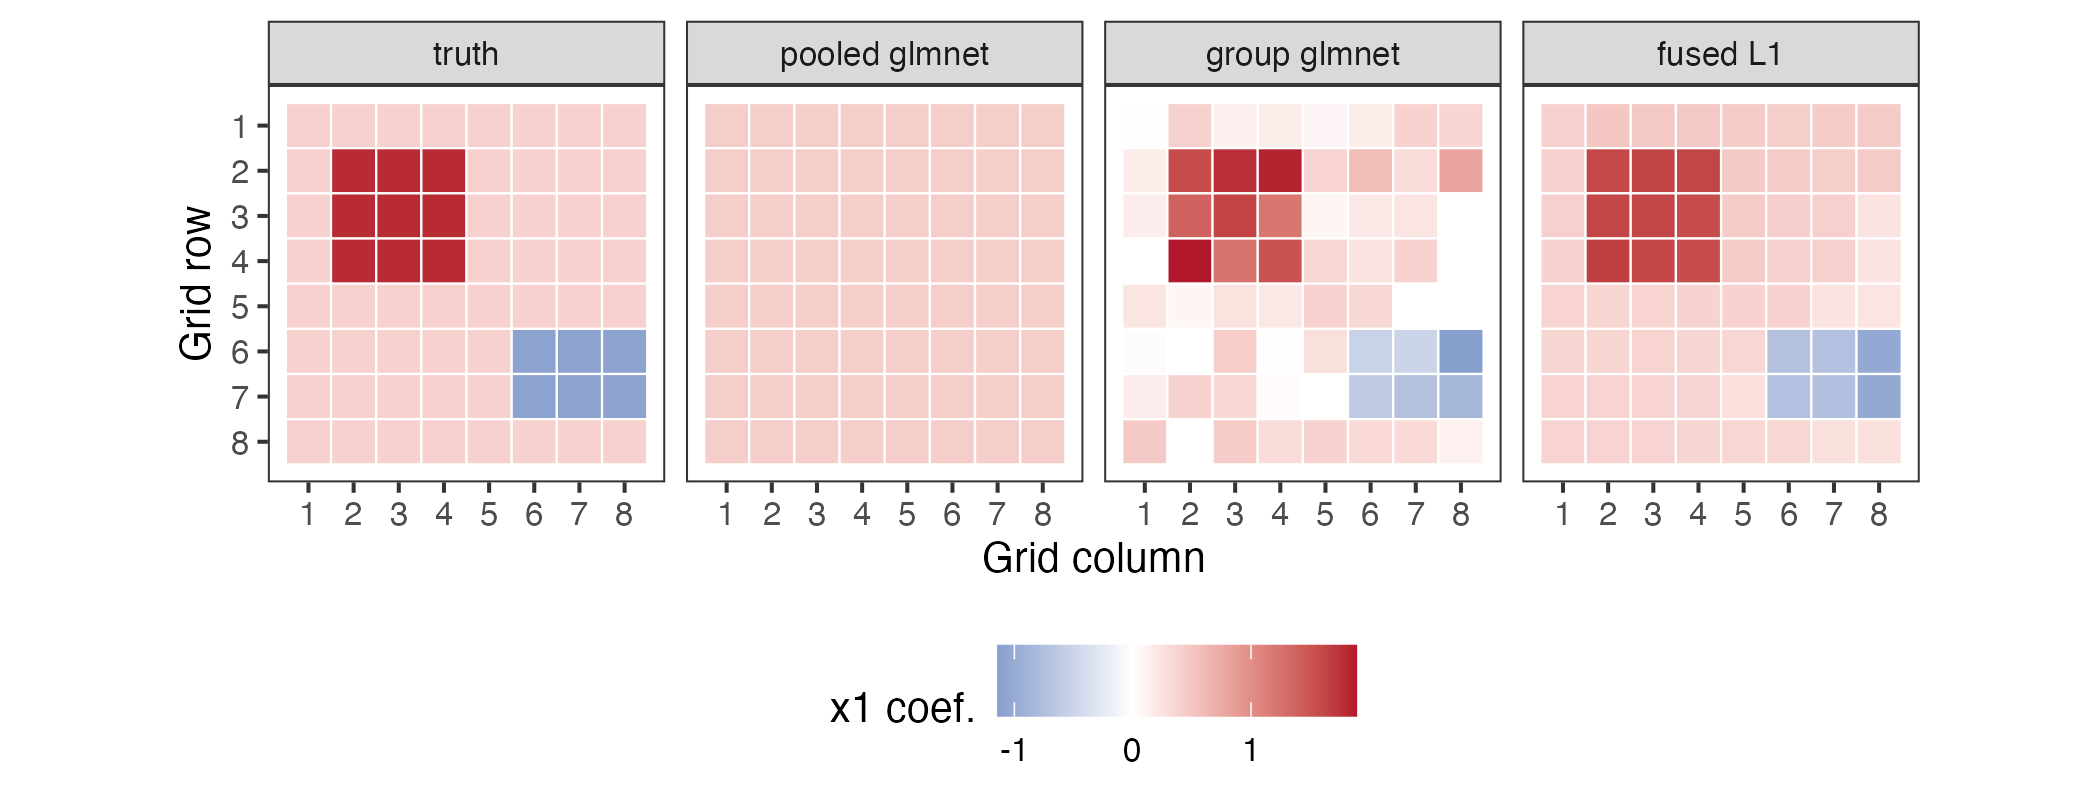
\includegraphics[width=.95\textwidth]{figures/spatial_hotspot_fused_vs_glmnet.png}
  \caption{Controlled spatial-hotspot example comparing fused regression with
  \texttt{glmnet} baselines on an $8\times 8$ group grid. The panels show the
  first coefficient over the spatial graph. Pooled \texttt{glmnet} smooths
  away the hotspots, group-specific \texttt{glmnet} gives noisy fragmented
  regions, and fused L1 recovers the contiguous hotspot structure.}
  \label{fig:spatial-hotspot-glmnet}
\end{figure}

\begin{table}[t]
\centering
\scriptsize
\caption{Synthetic structured-heterogeneity comparisons against
\texttt{glmnet} baselines. The relative coefficient error is Frobenius error
divided by the true coefficient Frobenius norm. CP distance is mean distance
from true changepoints to the nearest estimated large jump. Boundary F1 is
computed on graph edges by thresholding adjacent coefficient-vector
differences.}
\label{tab:structured-glmnet}
\begin{tabular}{@{}>{\raggedright\arraybackslash}p{0.16\textwidth}
>{\raggedright\arraybackslash}p{0.19\textwidth}rr
>{\raggedright\arraybackslash}p{0.28\textwidth}@{}}
\toprule
Example & Method & Test RMSE & Coef. rel. error & Structure metric \\
\midrule
Changepoint & pooled \texttt{glmnet} & 1.957 & 0.848 & CP dist. 28; 0 jumps \\
Changepoint & group \texttt{glmnet} & 0.915 & 0.279 & CP dist. 0; 59 jumps \\
Changepoint & fused L1 & 0.708 & 0.079 & CP dist. 0; 2 jumps \\
Spatial hotspot & pooled \texttt{glmnet} & 1.417 & 0.845 & boundary F1 0.000; 0 jumps \\
Spatial hotspot & group \texttt{glmnet} & 0.986 & 0.443 & boundary F1 0.325; 103 jumps \\
Spatial hotspot & fused L1 & 0.813 & 0.196 & boundary F1 1.000; 20 jumps \\
\bottomrule
\end{tabular}
\end{table}

\subsection{L1 Accuracy and Efficiency}

Figure~\ref{fig:l1-accuracy} compares L1 test RMSE against the legacy L1
baseline. The exact operator method matches the legacy prediction error to
numerical precision across the completed benchmark summary: the maximum
absolute percent difference in mean RMSE is below $10^{-5}$ percent. This is
expected because the operator form is an exact representation of the same
active-edge objective.

The chain-specialized method is faster but approximate. Its median RMSE
increase relative to the legacy method is 2.02\% in the completed L1 summary,
with larger losses on some datasets. This behavior is consistent with the
method's design: replacing a graph by a chain changes the fusion prior.

\begin{figure}[t]
  \centering
  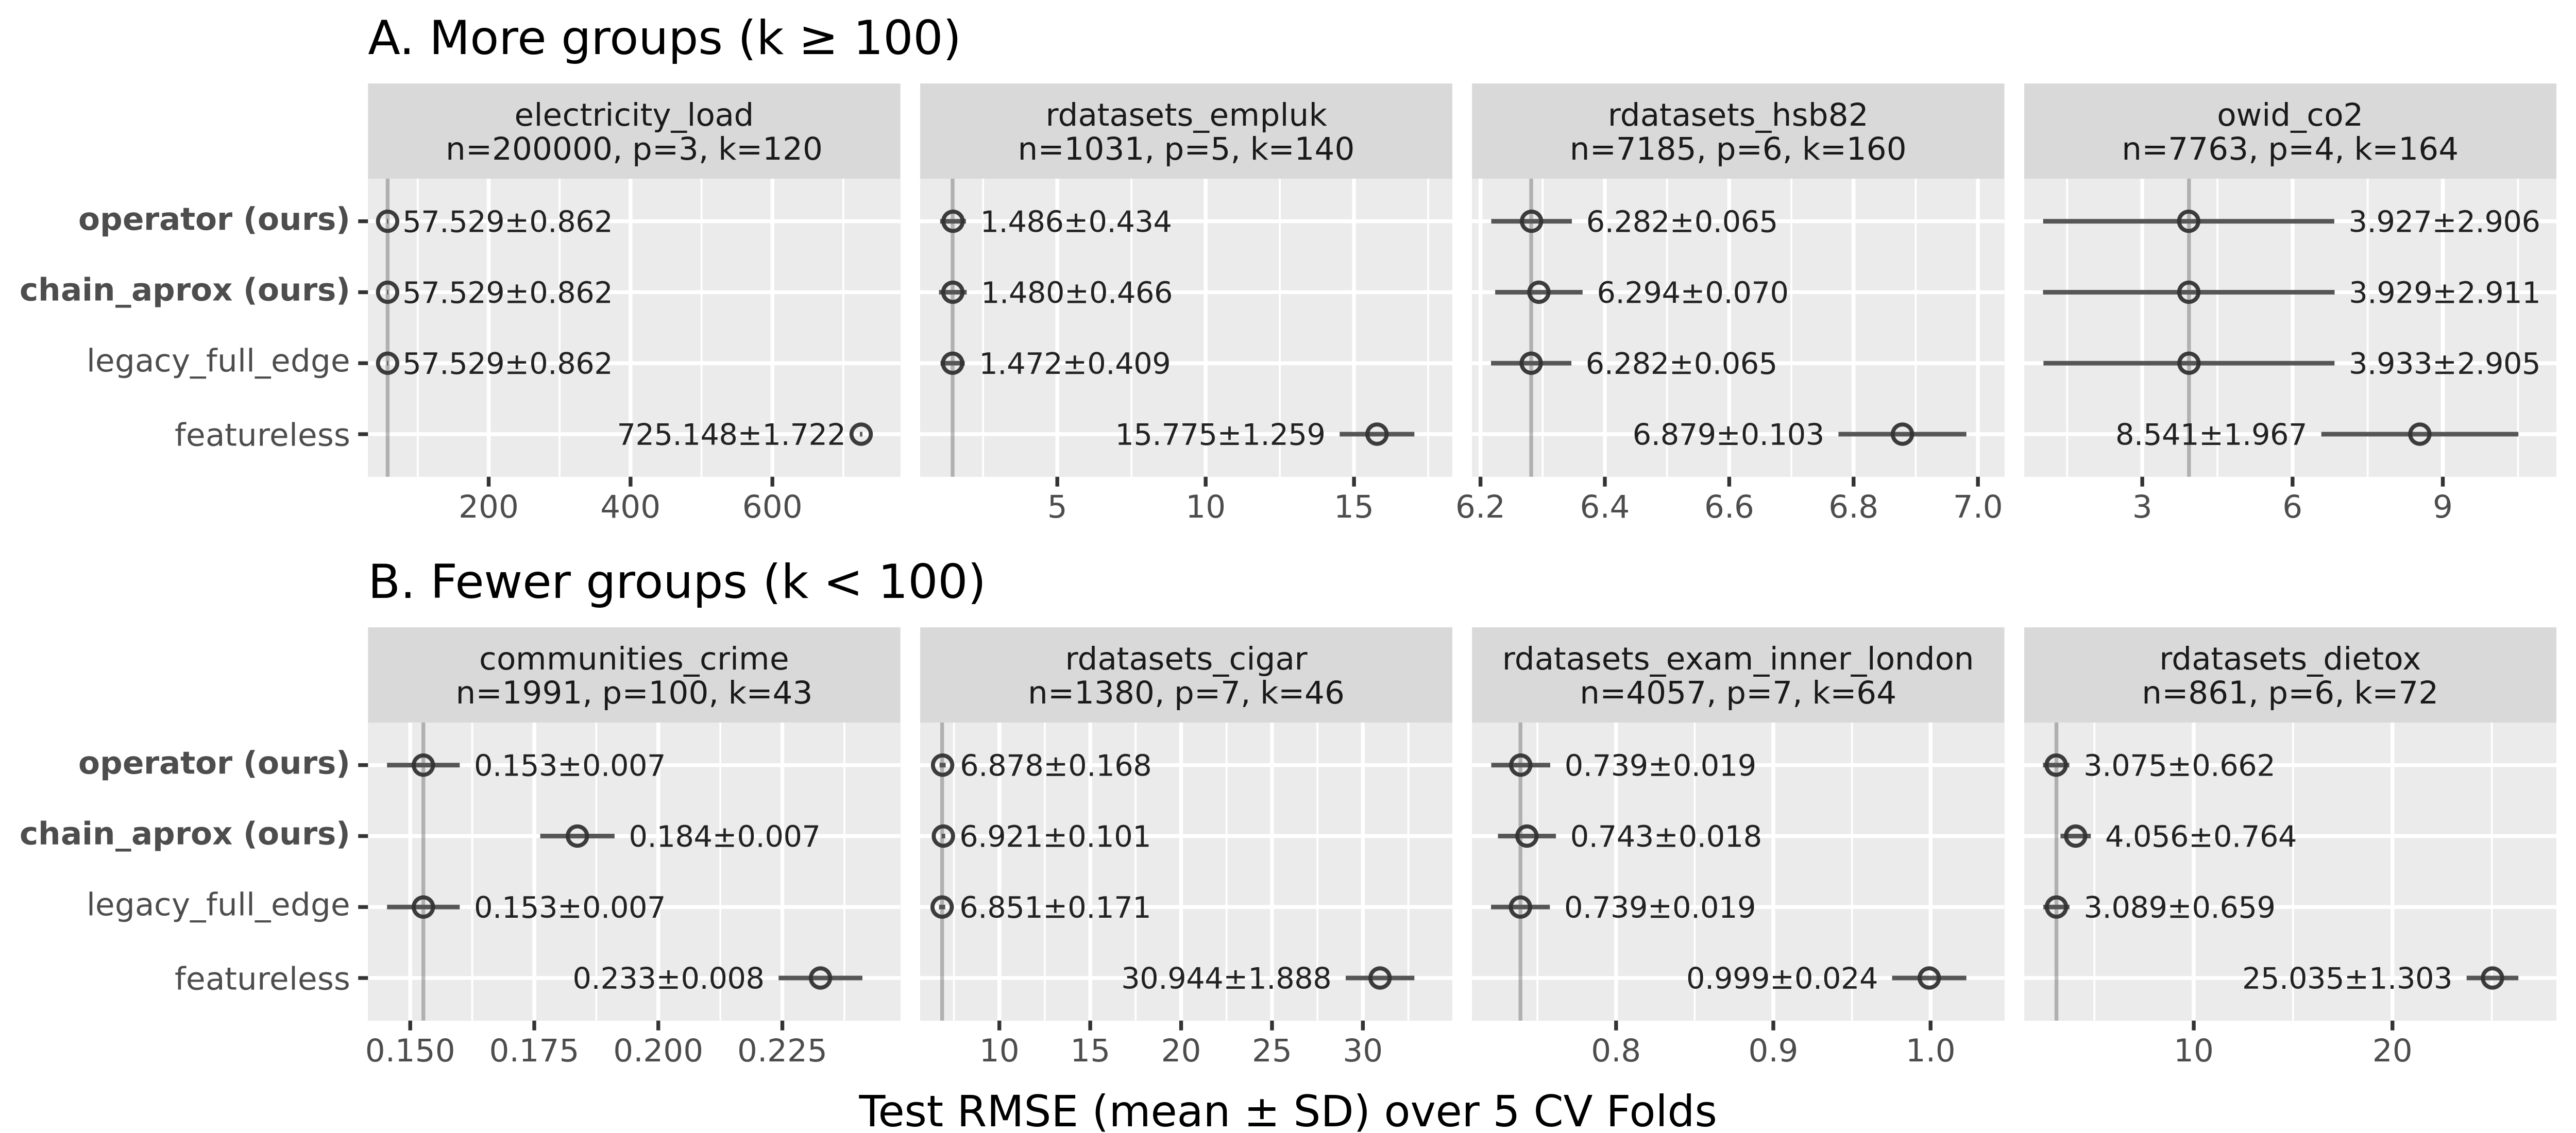
\includegraphics[width=\textwidth]{figures/hpc_figure5_combined_k_regimes.png}
  \caption{L1 prediction accuracy relative to the legacy L1 solver on the
  main benchmark panel. The exact operator solver preserves the legacy RMSE,
  while the chain-specialized approximation trades graph fidelity for speed.}
  \label{fig:l1-accuracy}
\end{figure}

Figure~\ref{fig:l1-timing} summarizes L1 fit time across group-count regimes.
In the completed L1 summary, the exact operator method has a median speedup of
2.26x over the legacy implementation, with speedups ranging from 0.68x to
7.65x. The one slowdown occurs on a small benchmark where overhead dominates
the savings from active-edge representation. Median peak memory decreases by
10.7\%.

The chain-specialized approximation has a median runtime speedup of 3.26x.
Its runtime gains are larger because it always uses only $k-1$ fusion edges.
Its median peak-memory reduction is 4.6\%, but memory gains vary by dataset
because the implementation still carries fixed R and matrix overheads.

\begin{figure}[t]
  \centering
  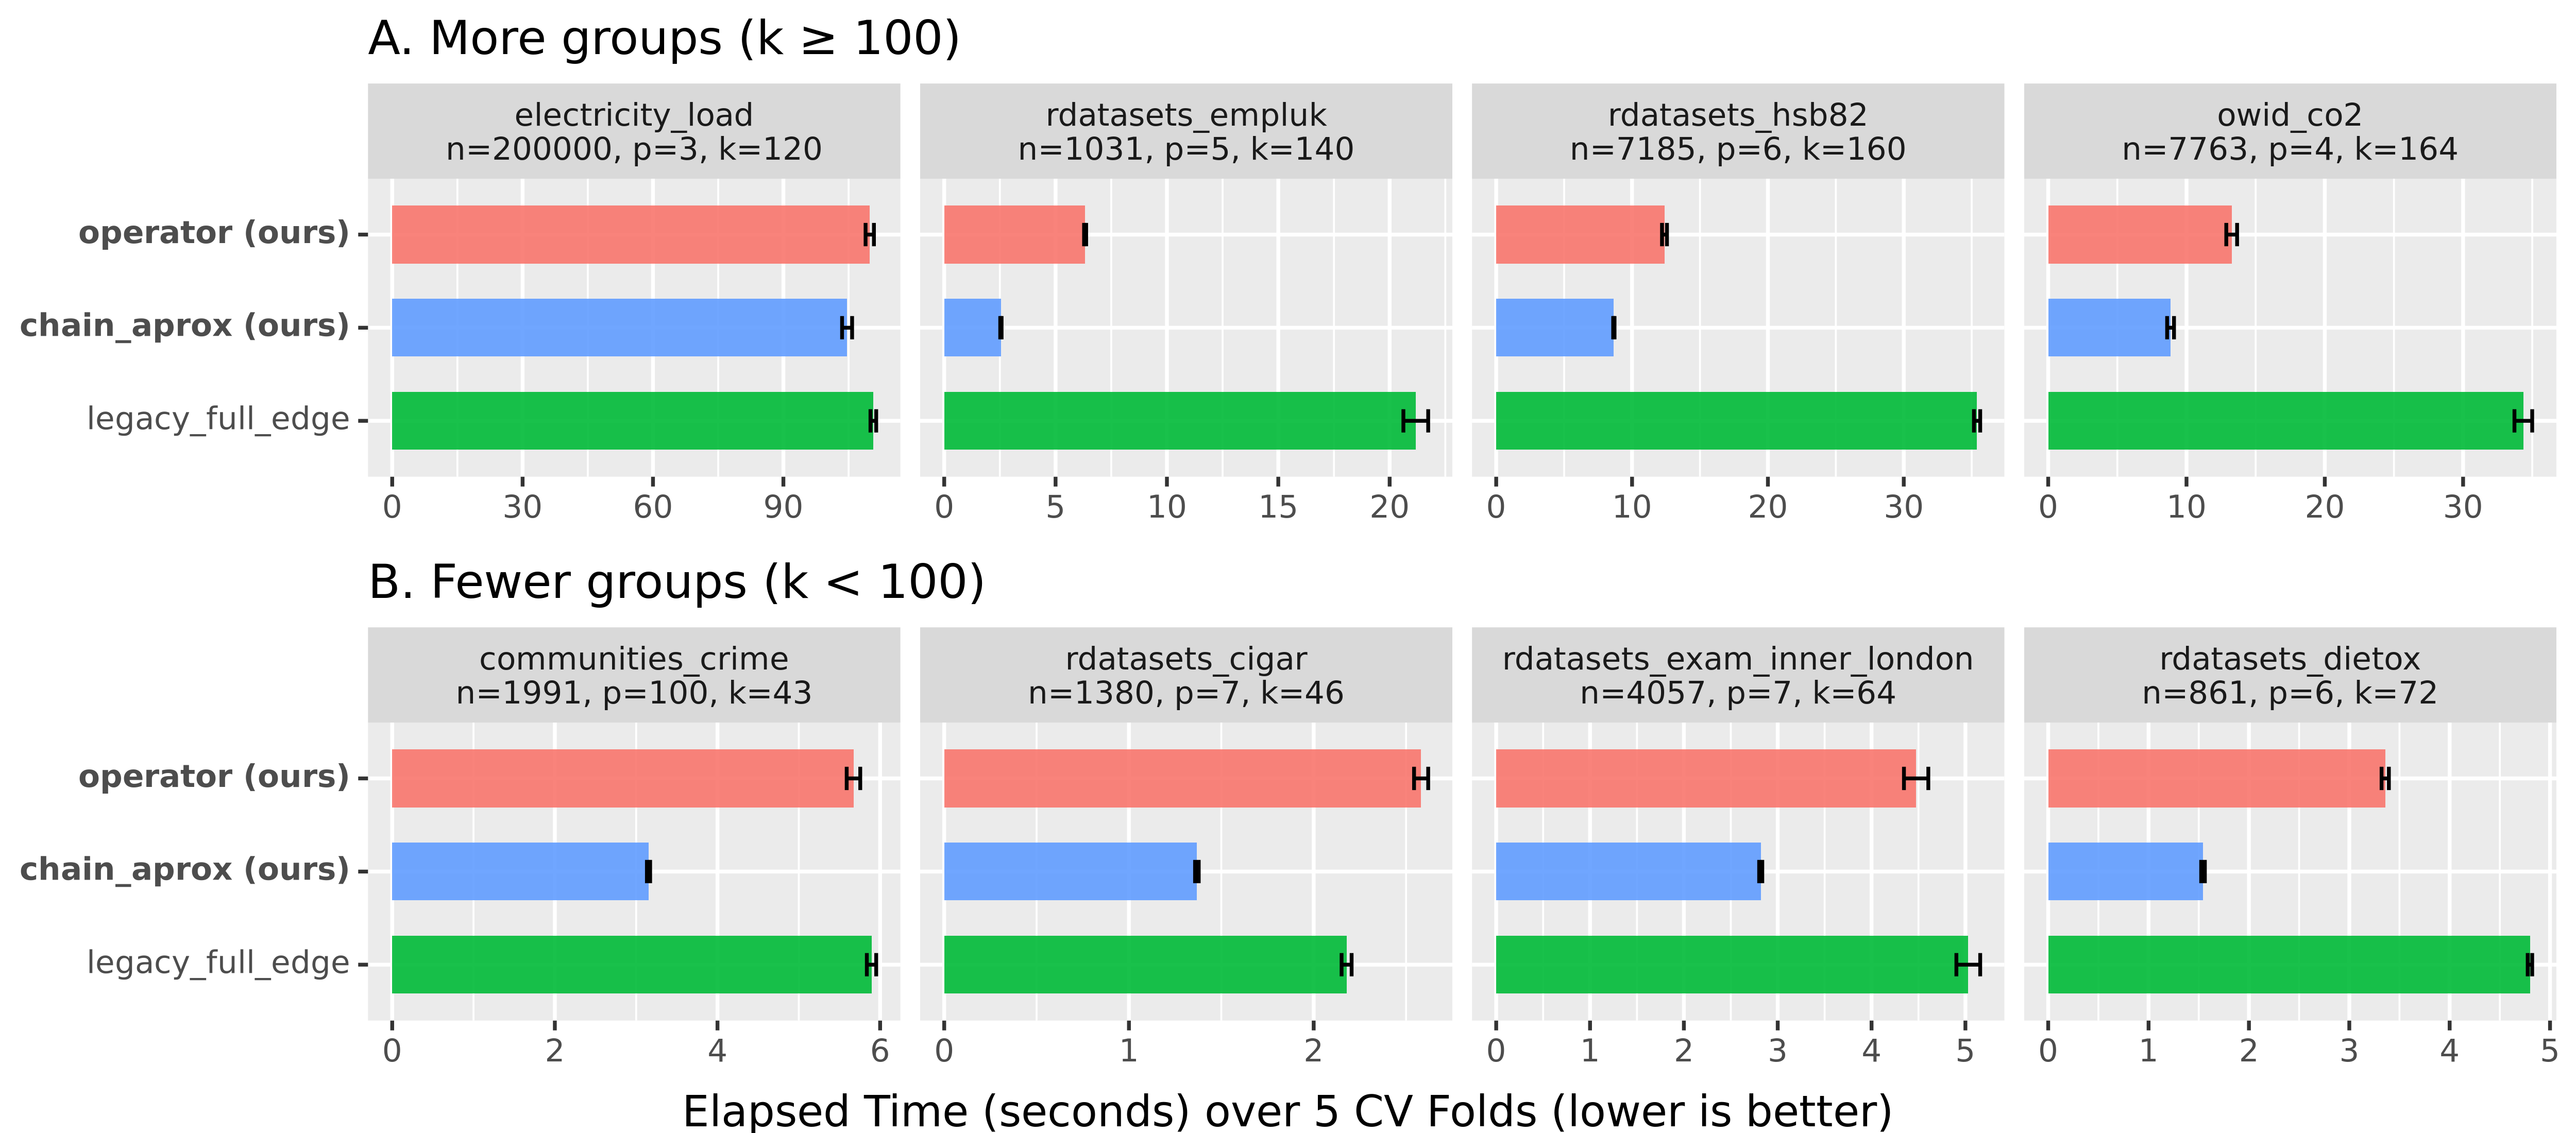
\includegraphics[width=\textwidth]{figures/hpc_l1_timing_boxplot_combined_k_regimes.png}
  \caption{L1 fit time by solver and group-count regime. Active-edge methods
  reduce the cost of graph fusion when the graph is sparse.}
  \label{fig:l1-timing}
\end{figure}

\begin{figure}[t]
  \centering
  
\includegraphics[width=.48\textwidth]{figures/hpc_l1_efficiency_diff_vs_old_l1_operator.png}
  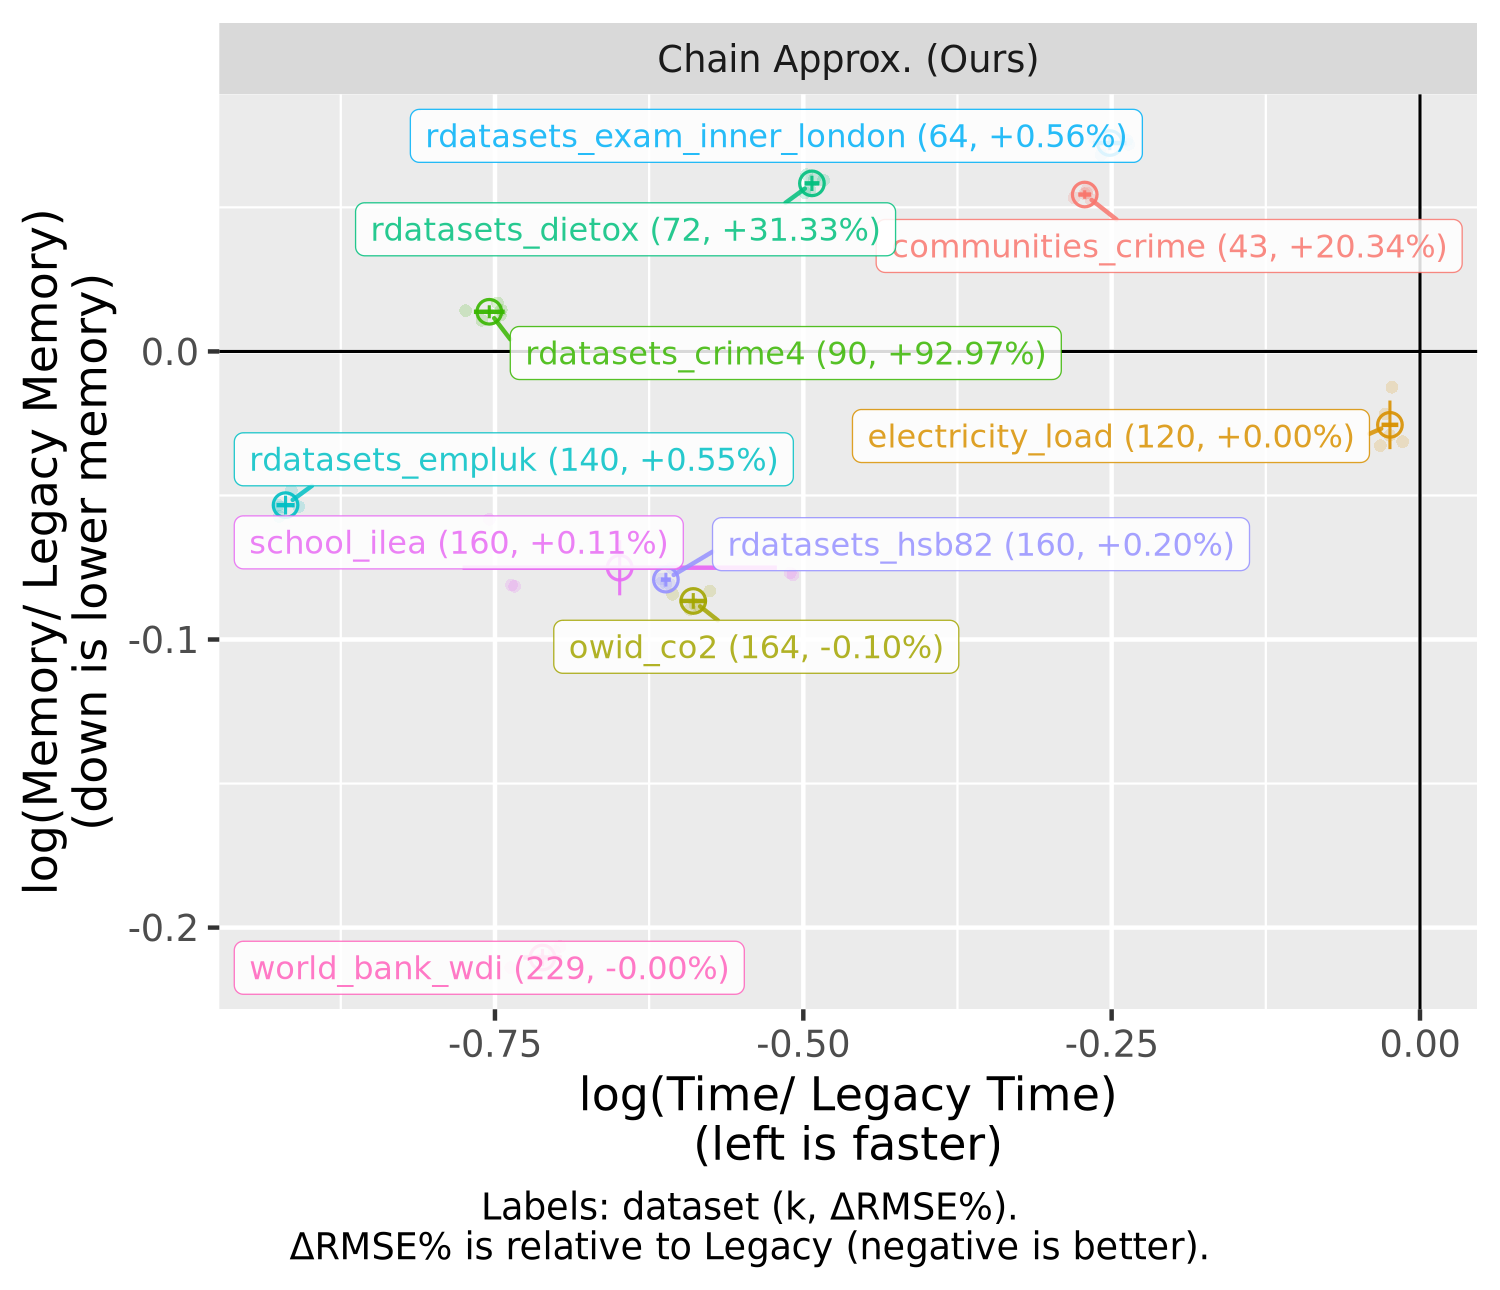
\includegraphics[width=.48\textwidth]{figures/hpc_l1_efficiency_diff_vs_old_l1_chain_specialized_full_plus4.png}
  \caption{L1 efficiency relative to the legacy solver. Left: exact operator.
  Right: chain-specialized approximation.}
  \label{fig:l1-efficiency}
\end{figure}

\subsection{L2 Accuracy and Efficiency}

The L2 active-edge builder is designed to preserve the legacy augmented
objective while avoiding all-pair construction. Across the 19-dataset L2
summary, \texttt{new\_l2} has median percent RMSE difference of -0.025\%
relative to \texttt{old\_l2}. The largest observed RMSE increase is 0.134\%,
while several datasets show small decreases in RMSE from the active-edge
construction and numerical path. The median fit-time speedup is 14.9x across
all 19 datasets and 105.3x on the 11 datasets with at least 50 groups. Median
peak fit-worker memory decreases by 19.9\% across the full L2 panel.

\begin{figure}[t]
  \centering
  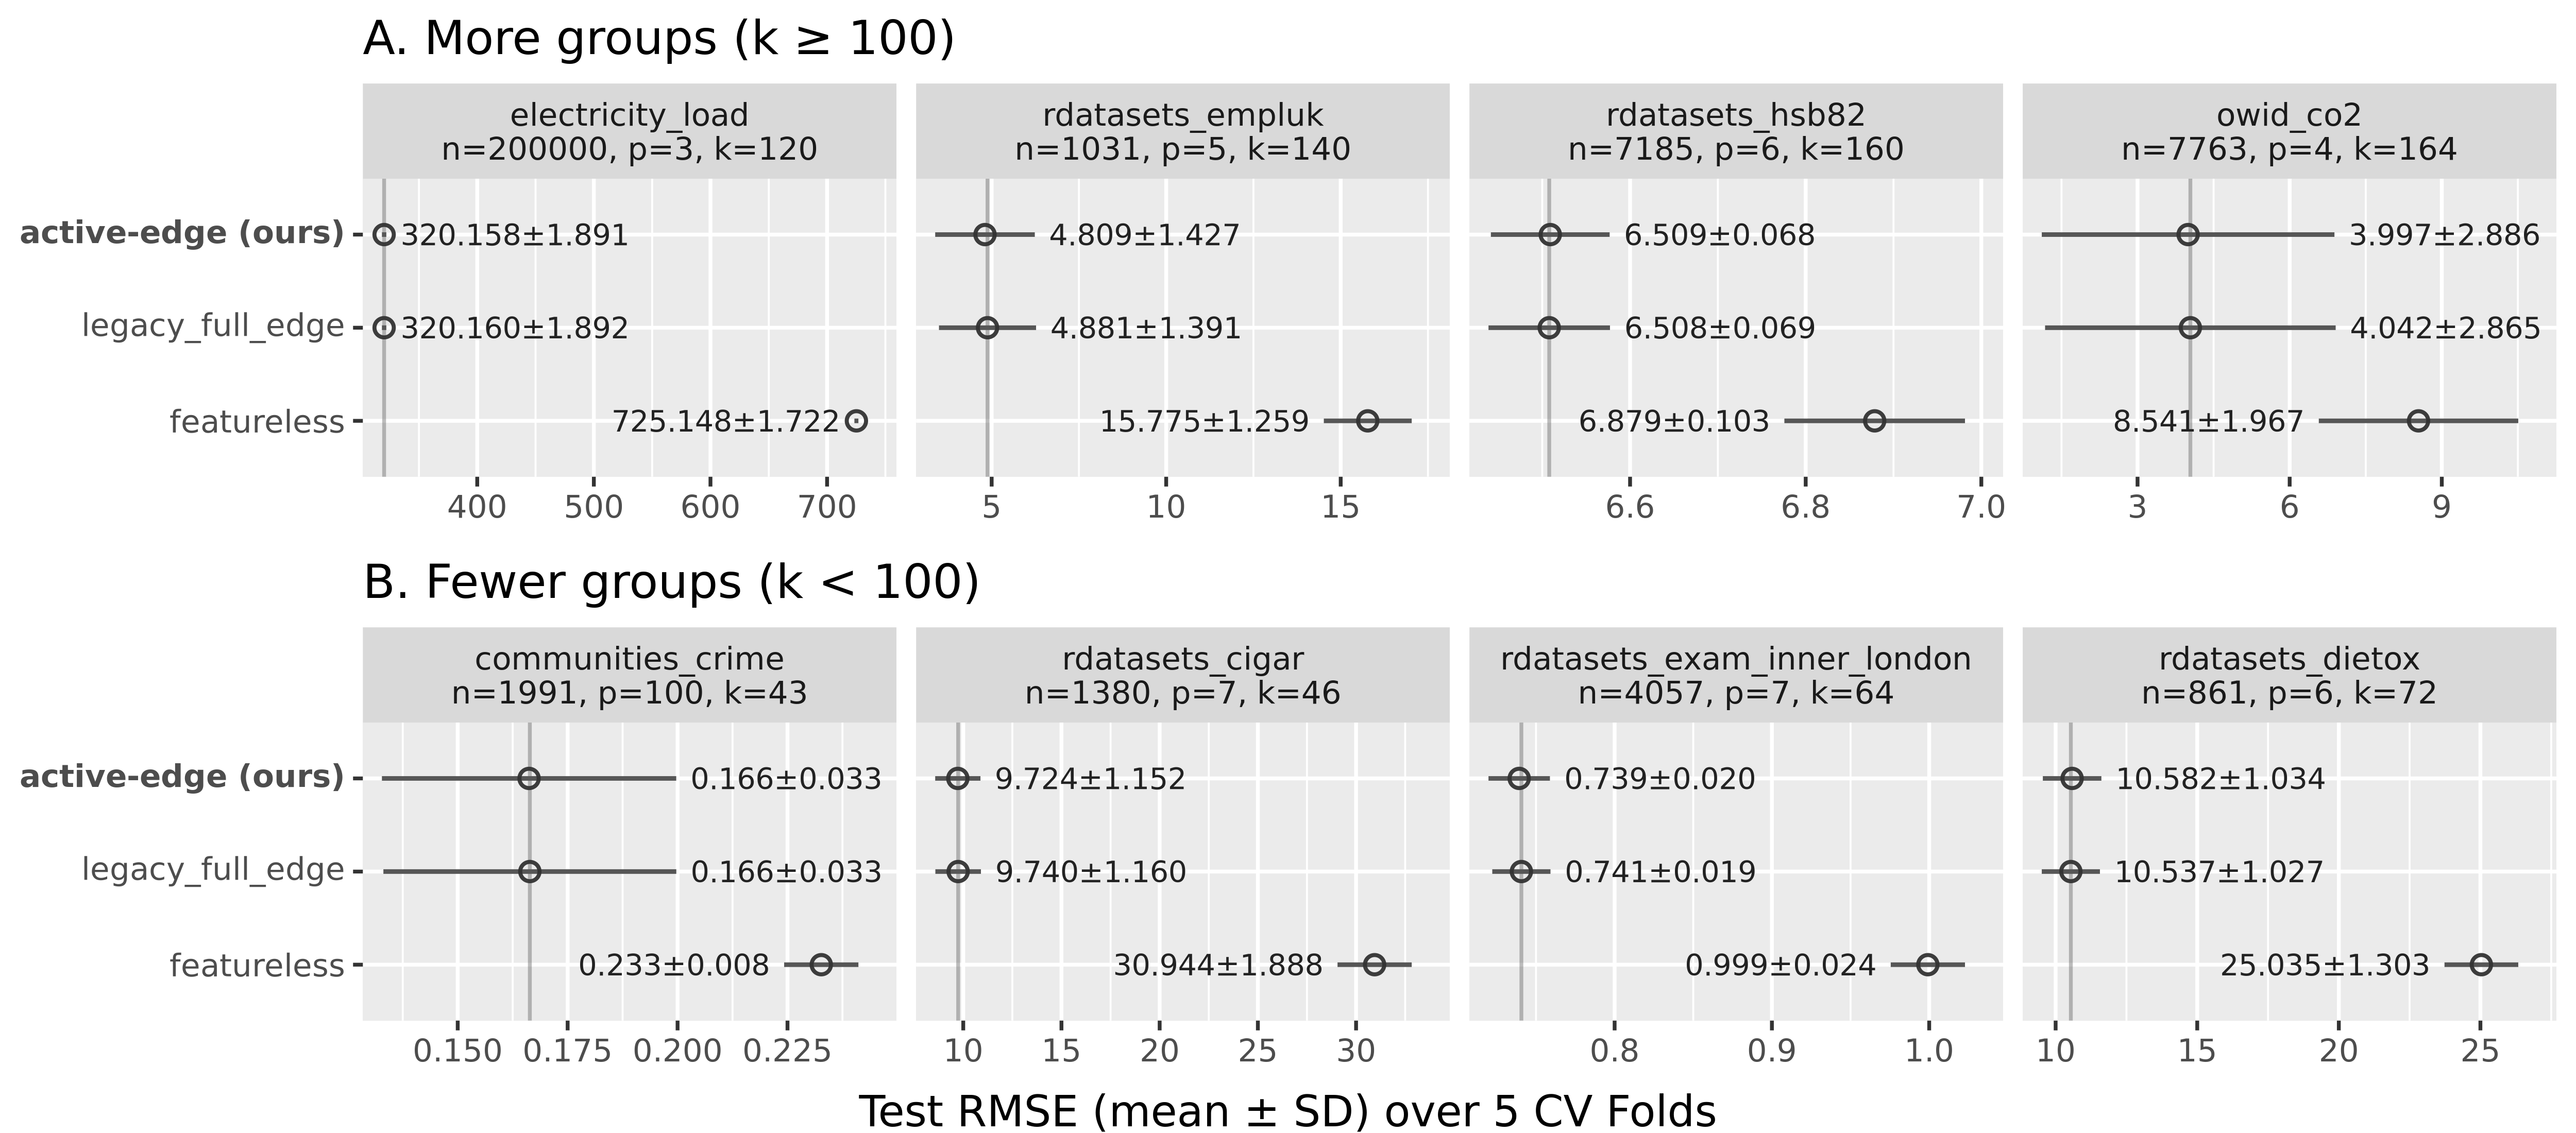
\includegraphics[width=\textwidth]{figures/hpc_l2_figure5_combined_k_regimes.png}
  \caption{L2 prediction accuracy relative to the legacy L2 augmented-design
  solver across the benchmark panel.}
  \label{fig:l2-accuracy}
\end{figure}

\begin{figure}[t]
  \centering
  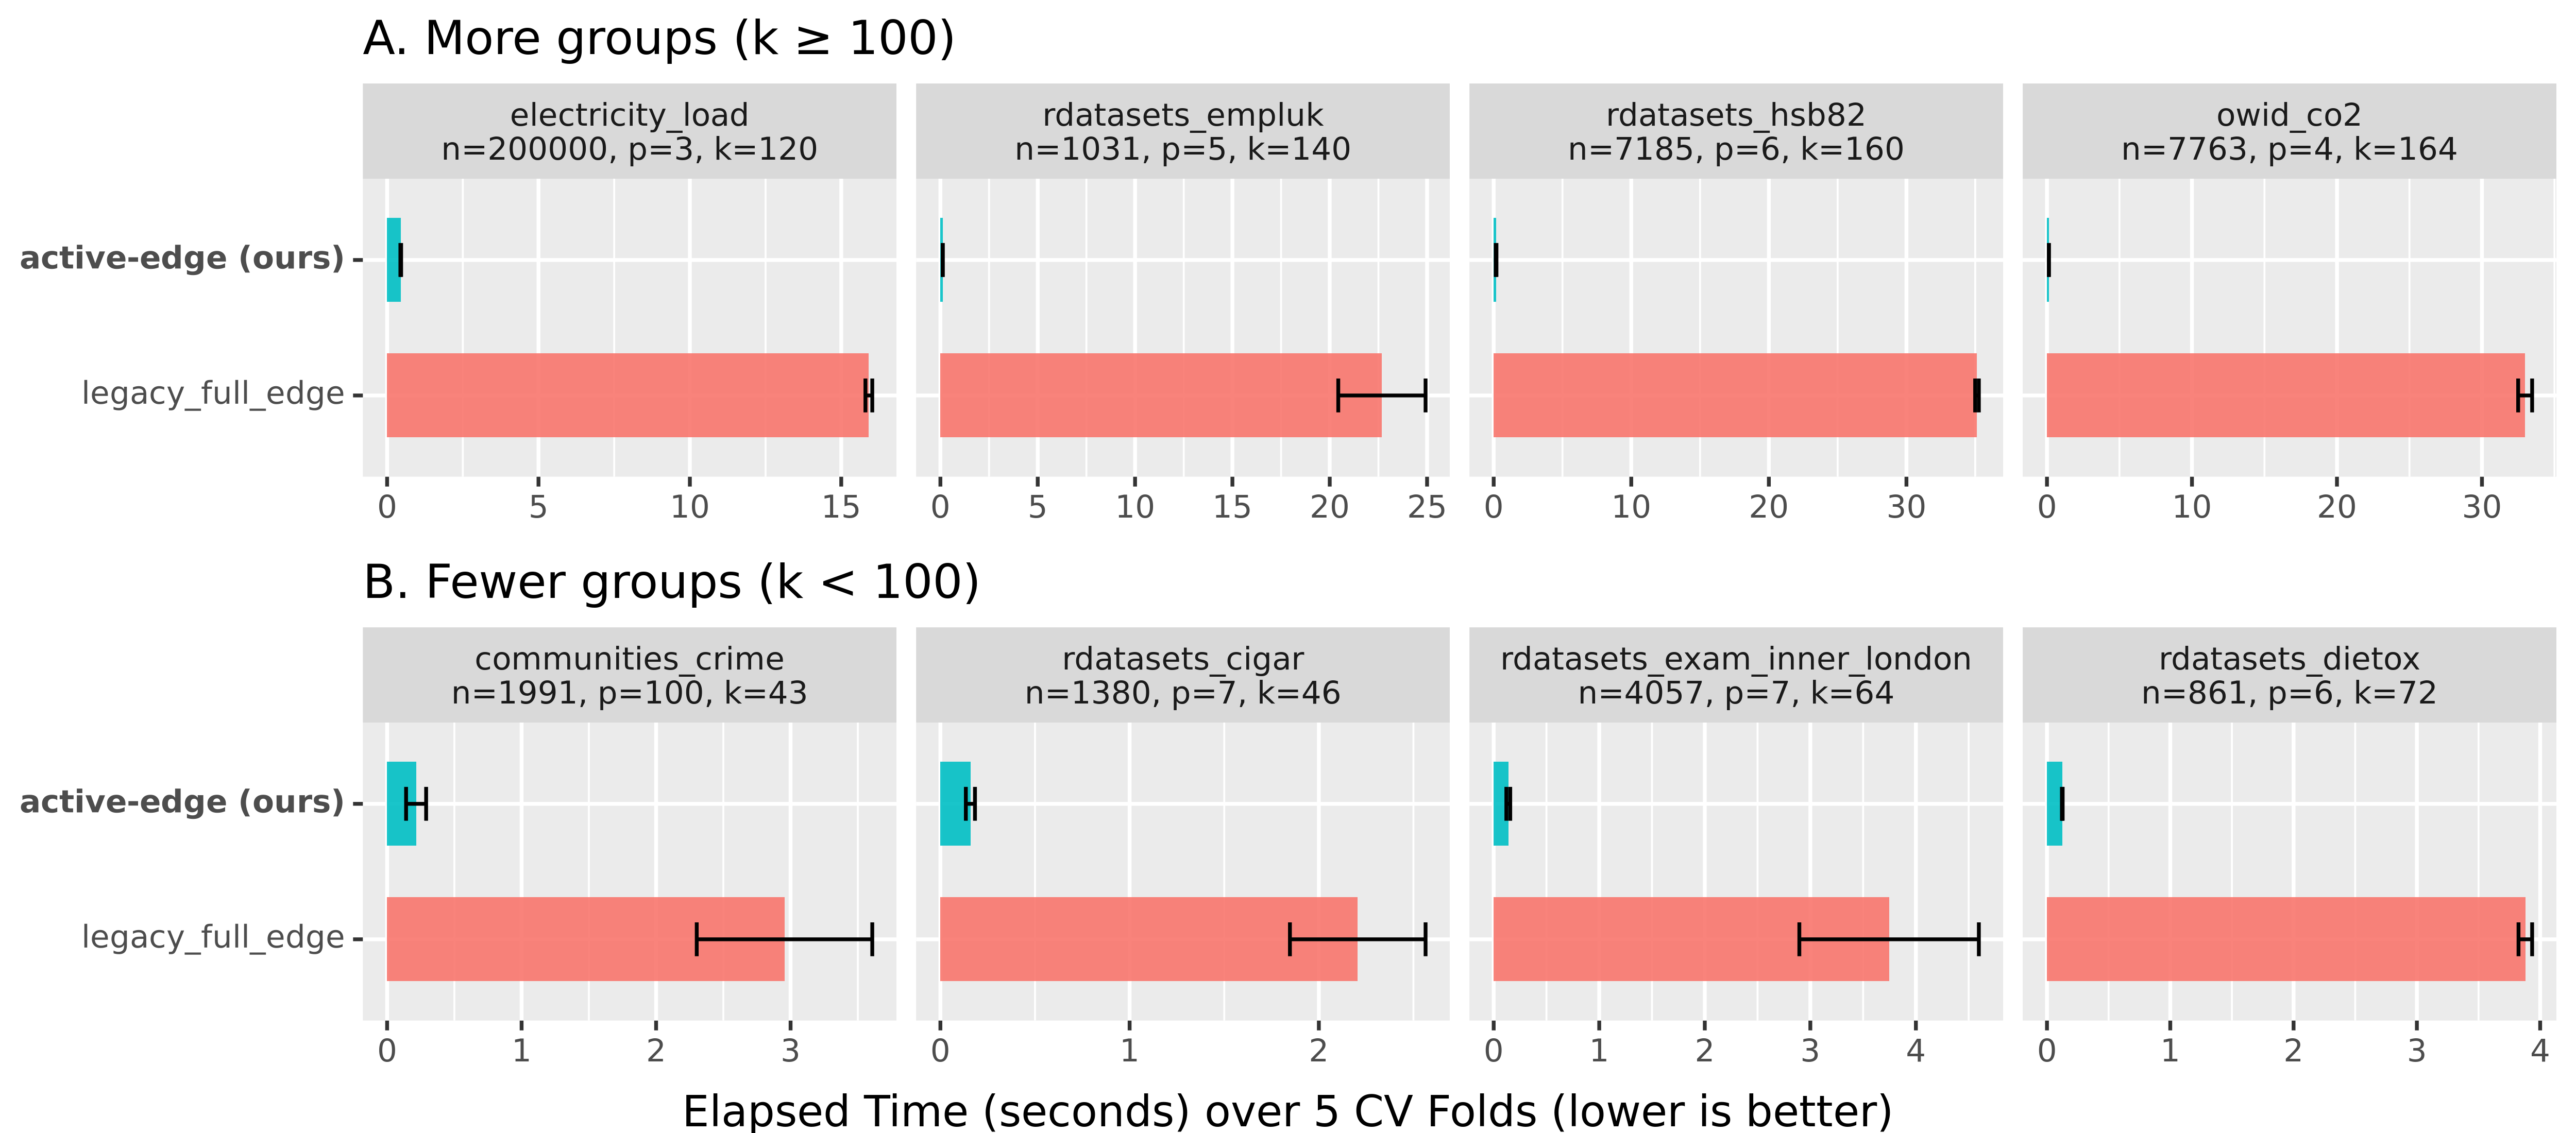
\includegraphics[width=\textwidth]{figures/hpc_l2_timing_boxplot_combined_k_regimes.png}
  \caption{L2 fit time by solver and group-count regime. The active-edge
  builder reduces augmented-design construction when the graph is sparse.}
  \label{fig:l2-timing}
\end{figure}

\begin{figure}[t]
  \centering
  
\includegraphics[width=.58\textwidth]{figures/hpc_l2_efficiency_diff_vs_old_l2_new_l2.png}
  \caption{L2 efficiency of active-edge construction relative to the legacy
  L2 construction.}
  \label{fig:l2-efficiency}
\end{figure}

\subsection{Synthetic Scaling Experiments}

The repository also includes synthetic scaling experiments generated by the
\texttt{atime} benchmark scripts. These experiments isolate solver scaling
under controlled changes to the number of groups and graph structure. They
support the same qualitative conclusion as the real-data benchmarks: avoiding
all-pair graph construction matters most when $k$ grows and the graph remains
sparse.

\section{Discussion}

The main lesson is representational: graph-aware statistical models should
carry graph sparsity into the optimizer. When the graph has $m$ edges, an
implementation that constructs $O(k^2)$ pairwise constraints can lose the
computational advantage of modeling with a sparse graph. This is a general
issue for edge-penalized regression, not only for \fuserplus. Any method whose
penalty decomposes over graph edges can pay an unnecessary quadratic cost if
the graph is represented by a complete set of candidate pairs. The L1 operator
and L2 active-edge builders recover the intended $O(pm)$ fusion
representation while preserving the original objective in the exact cases.

The exact L1 operator is the safest default among the proposed L1 variants.
It preserves the same fitted objective as the legacy active-edge formulation
and gives substantial median runtime and memory improvements on the completed
benchmark summary. The chain-specialized solver is more aggressive. It is best
viewed as an approximation for exploratory or large-scale settings where a
small loss in predictive accuracy is acceptable.

The solver representation aligns the computational graph with the modeling
graph. Edge-explicit L1 fusion updates, blocked edge processing, DFS/MST chain
approximation, and active-edge L2 matrix construction are instances of that
representation. Propositions
\ref{prop:l1-equivalence} and \ref{prop:l2-equivalence} identify the exact
cases where the new representations preserve the legacy objective. The
chain-specialized method is separated from those exact methods because
replacing a graph by a chain changes the fusion geometry and should be
interpreted as an approximation.

The empirical evidence is strongest for the exact L1 operator and active-edge
L2 construction. The chain variant is included because it is a useful solver
mode in the package, but it involves an additional graph-approximation choice.
For that reason, the recommended default for sparse L1 fusion is the exact
active-edge operator, with chain-specialized fitting reserved for exploratory
or memory-constrained settings.

There are three important limitations. First, the paper analyzes
representation equivalence and graph-construction complexity, but it does not
introduce new statistical guarantees for fused regression estimators. The
statistical behavior is inherited from the underlying fused-lasso and
graph-guided regression objectives. Second, the largest gains occur when the
user-supplied or data-derived graph is sparse. If the modeling graph is close
to complete, the active-edge representation has little edge-count advantage.
Third, the software is an R implementation, so small problems can be dominated
by fixed interpreter, allocation, and \texttt{glmnet} overheads. These limits
explain the occasional small-benchmark slowdown and motivate the recommendation
to use the exact operator as the default sparse-graph path rather than as a
universal speed guarantee.

\section{Reproducibility}

The implementation is in the \fuserplus R package, version 0.1.0
(\texttt{DESCRIPTION}), evaluated from repository commit
\texttt{99c69ae32a93e018852c6facc2d3f1e27a1068c5}. The benchmark environment
used R version 4.5.2 (2025-10-31). The package contains R documentation under
\path{man}, a vignette under \path{vignettes}, and \texttt{testthat} tests for
the legacy L1/L2 solvers, Rcpp consistency, eigenvalue helpers, and the new L2
builder. The exported namespace includes the legacy user-facing solvers and
helpers, while the benchmarked active-edge routines are implemented as package
functions and invoked by the benchmark wrappers. The solver routines discussed
in this paper are:
\begin{itemize}
\item \path{fusedLassoProximal}: legacy L1 fusion.
\item \path{fusedLassoProximalNewOperator}: active-edge L1 fusion.
\item \path{fusedLassoProximalChainSpecialized}: chain L1 approximation.
\item \path{fusedL2DescentGLMNet}: legacy L2 fusion.
\item \path{fusedL2DescentGLMNetNew}: active-edge L2 fusion.
\end{itemize}
Benchmark scripts are stored under \path{scripts/benchmark_*.R} and
\path{scripts/hpc}. Processed dataset metadata and licensing notes are stored
under \path{data/processed}. The HPC scripts include a manifest builder, a
single-row runner, an aggregator, memory-tier splitting, and a SLURM array
template using one CPU per task with conservative 24-hour and 32GB defaults.
The exact CSV files used for the results in this paper are:
\begin{itemize}
\item \path{build/hpc/final_test_summary.csv} for the 12-dataset L1 panel.
\item \path{build/hpc/l2_knn/final_test_summary.csv} for the 19-dataset L2
panel.
\item \path{build/hpc/l2_knn/final_test_summary_k_ge_50.csv} for the
large-group L2 subset.
\item \path{build/changepoint/fused_vs_glmnet_summary.csv} for the synthetic
changepoint comparison.
\item \path{build/spatial_hotspot/fused_vs_glmnet_summary.csv} for the
synthetic spatial-hotspot comparison.
\end{itemize}

The manifest-driven benchmark pipeline can be rerun with commands of the
following form:
\begin{verbatim}
Rscript scripts/hpc/build_test_manifest.R \
  --objective l1 \
  --methods old_l1,operator,chain_specialized \
  --out_csv build/hpc/test_manifest.csv \
  --results_dir build/hpc/test_jobs

Rscript scripts/hpc/run_test_job.R \
  --manifest_csv build/hpc/test_manifest.csv \
  --row_id 1

Rscript scripts/hpc/aggregate_test_results.R \
  --manifest_csv build/hpc/test_manifest.csv \
  --out_all_csv build/hpc/test_results_all.csv \
  --out_summary_csv build/hpc/final_test_summary.csv
\end{verbatim}
The L2 panel uses the same pipeline with \texttt{--objective l2},
\texttt{--methods old\_l2,new\_l2}, and output paths under
\path{build/hpc/l2_knn}. The synthetic changepoint comparison is generated by
\path{scripts/benchmark_changepoint_fused_vs_glmnet.R}, and the spatial-hotspot
comparison is generated by
\path{scripts/benchmark_spatial_hotspot_fused_vs_glmnet.R}. The synthetic
scaling experiments are generated by the \texttt{benchmark\_atime\_*} scripts
under \path{scripts}. The paper source can be rebuilt from
\path{publication/paper1/fuserplus_jmlr.tex} with the JMLR style file in the
same directory.

\section{Conclusion}

\fuserplus demonstrates that sparse-graph construction can materially improve
grouped fused regression solvers without changing the statistical model. The
exact L1 operator and active-edge L2 augmented-design builder preserve the
legacy objectives while reducing avoidable all-pairs graph costs. The
chain-specialized L1 approximation provides an additional high-efficiency mode
when the user is willing to trade graph fidelity for speed. These changes make
fused regression more practical for grouped datasets with many subgroups and
sparse relationships.

\acks{Daniel Agyapong is affiliated with Northern Arizona University. The
author thanks the maintainers of the public datasets and R packages used in
the benchmark suite.}

\bibliography{fuserplus_refs}

\end{document}
